% ----- Start of translated content from: part_01.tex -----

\documentclass[11点, A4纸, 单面]{article}

% --- 必要的包 ---
\usepackage{graphicx} % 用于插入图片(标志)
% 调整边距以增加页眉空间
\usepackage[a4paper, top=4cm, bottom=2.5cm, left=2.5cm, right=2.5cm, headheight=1.2cm, headsep=1.5cm]{geometry}
\usepackage{xcolor} % 用于定义和使用自定义颜色
\usepackage{titlesec} % 用于自定义章节标题
\usepackage{enumitem} % 用于自定义列表
\usepackage{hyperref} % 用于创建内外部链接
\usepackage{ragged2e} % 用于改善文本对齐
\usepackage{lettrine} % 用于首字母
\usepackage{fancyhdr} % 用于自定义页眉页脚
\usepackage{tabularx} % 用于定义宽度的表格
\usepackage{amsfonts} % 用于数学符号(如果需要)
\usepackage{amsmath}
\usepackage[utf8]{inputenc}
\usepackage{graphicx}
\usepackage{booktabs}
\usepackage{tikz}
\usepackage{pgfplots}
\usepackage{float}
\usepackage{eurosym}
\usepackage{microtype}
\usepackage{siunitx} 
\pgfplotsset{compat=1.18}
% --- 字体和语言设置(需要 XeLaTeX) ---
\usepackage{fontspec}
\usepackage{xeCJK}
\usepackage{multirow}
\usepackage{booktabs,longtable,siunitx,ragged2e,placeins} 

\def\UrlBreaks{\do\.\do\/\do\-\do\_\do\?\do\&} % 允许在URL中断行
\newcolumntype{L}{>{\raggedright\arraybackslash}X} % 定义宽度可变且左对齐的列


% 直接从本地文件加载字体,指定不同字重
% 这是最稳健的方法
% 确保.ttf文件在名为“fonts”的子文件夹中
\setmainfont{NotoSans-Regular.ttf}[
    Path = ./fonts/,
    BoldFont = NotoSans-Bold.ttf,
    ItalicFont = NotoSans-Italic.ttf,
    BoldItalicFont = NotoSans-BoldItalic.ttf
]
\setCJKmainfont{NotoSansSC-Regular.ttf}[
    Path = ./fonts/,
    BoldFont = NotoSansSC-Bold.ttf,
    ItalicFont = NotoSansSC-Regular.ttf
]
% 定义一个新的“light”字体,用于个性化需求
\newfontfamily\lightfont{NotoSans-Light.ttf}[
    Path = ./fonts/,
    ItalicFont = NotoSans-LightItalic.ttf
]



% --- 品牌颜色定义(可自定义) ---
\definecolor{PrimaryColor}{HTML}{6A4C9C}   % 主要颜色(例如:紫色)
\definecolor{SecondaryColor}{HTML}{2A2F45} % 次要颜色(例如:深蓝色)
\definecolor{AccentColor}{HTML}{8E7CC3}    % 强调色
\definecolor{DarkGray}{HTML}{343a40}      % 深灰色用于文本

% --- hyperref 设置 ---
\hypersetup{
    colorlinks=true,
    linkcolor=PrimaryColor,
    filecolor=AccentColor,      
    urlcolor=SecondaryColor,
    citecolor=AccentColor,
    pdftitle={商业计划},
    pdfpagemode=FullScreen,
}

% --- 章节标题自定义 ---
\titleformat{\section}
  {\normalfont\Large\bfseries\color{SecondaryColor}}
  {\thesection}{1em}{}
\titleformat{\subsection}
  {\normalfont\large\bfseries\color{PrimaryColor}}
  {\thesubsection}{1em}{}
\titleformat{\subsubsection}
  {\normalfont\normalsize\bfseries\color{AccentColor}}
  {\thesubsubsection}{1em}{}

% --- 页眉页脚设置 ---
\pagestyle{fancy}
\fancyhf{} % 清除所有页眉页脚栏位
% 设置左侧为文字,右侧为LOGO的页眉
\fancyhead[L]{\textcolor{PrimaryColor}{\small 商业计划书}}
\fancyhead[R]{
\includegraphics[height=0.8cm]{IntellyHub_Logo_Colored.png}}
\fancyfoot[C]{\textcolor{DarkGray}{\thepage}}
\renewcommand{\headrulewidth}{0.4pt}
\renewcommand{\footrulewidth}{0.4pt}
\renewcommand{\headrule}{\color{PrimaryColor}\hrule}
\renewcommand{\footrule}{\color{PrimaryColor}\hrule}


% --- 文档开始 ---
\begin{document}
% --- 标题页 ---
% 首页使用 'empty' 样式以免显示页眉
\thispagestyle{empty} 
\begin{titlepage}
    \centering
    \vspace{1cm}
    
    % 包含LOGO(将'logo.png'替换为你的文件)
    
\includegraphics[width=0.6\textwidth]{IntellyHub_Logo_Colored.png}
    
    \vspace{2.5cm}
    
    % 文档标题
    {\Huge\bfseries\color{PrimaryColor}商业计划书}
    
    \vspace{1.5cm}
    
    % 使用light字体的副标题示例
    {\Large\itshape\lightfont Automations That Think.}
    \vfill % 垂直空白弹性
     
    % 公司信息与日期
    {\large\bfseries\color{PrimaryColor}v2.08 \color{SecondaryColor}商业计划书}
    
    \vspace{0.5cm}
    
    {\large \today}
    
\end{titlepage}

% --- 目录 ---
\tableofcontents
\newpage

% --- 商业计划书目录 ---
\section{执行摘要}
IntellyHub 智联中枢是一个创新的AI工作流与智能体编排平台,旨在赋能中国企业构建、部署和管理复杂的AI驱动工作流及自主智能体。在中国加速迈入\textbf{人工智能时代}以及宏大的\textbf{《“十四五”数字经济发展规划》}背景下,我们的平台精准地填补了传统自动化工具与前沿AI框架之间的市场空白。
我们提供统一的企业级解决方案,无缝编排各种AI模型(大语言模型)、模型上下文协议(MCP)服务器、检索增强生成(RAG)流水线、自定义Python逻辑以及传统应用程序集成。IntellyHub创新的“可视化+代码”混合IDE和可扩展的插件系统,使AI工程师和DevOps团队无需具备深厚的 底层基础架构专业知识,即可快速将AI解决方案产品化并进行部署。
我们的核心战略是产品驱动增长(PLG)与销售驱动增长(SLG)相结合的混合模式。通过强大的免费版本和自助服务工具,我们旨在实现开发者社区内的爆炸式采纳和快速普及,并随着用户使用规模的扩大,将他们顺利转化为高价值的企业客户。
中国的AI自动化、AIOps和MLOps市场正经历着前所未有的爆发式增长。IntellyHub凭借其企业级的安全性、管理能力、可扩展性和以开发者为中心的灵活性,完美地处于这一历史性机遇的交汇点。
我们预计,通过我们为AI/ML工程用例量身定制的高价值SaaS和私有化部署模式,未来三年的用户和收入将实现强劲增长,助力中国企业在全球AI浪潮中占据领先地位。


\section{公司描述}
\subsection{使命宣言}
IntellyHub的使命是成为中国企业“智能数字化转型”的核心引擎。我们通过提供一个用于编排复杂工作流和自主智能体的统一平台,赋能企业释放人工智能的全部潜力。我们致力于打破传统自动化与前沿AI框架之间的壁垒,实现AI驱动解决方案的无缝集成和高效管理。


\subsection{愿景}
我们的愿景是,未来AI将深度融入企业运营的方方面面,使组织能够自动化复杂任务、优化决策制定并推动前所未有的商业创新。我们渴望成为世界领先的AI工作流编排平台,赋能开发者和企业构建能够变革行业、推动科学研究的智能系统,从而为中国的“数字中国”战略贡献力量。

\subsection{核心价值观}
\begin{itemize}
    \item \textbf{自主创新:}我们致力于持续的技术创新,不断探索AI与自动化的前沿领域,追求核心技术的资助可控。  
    \item \textbf{合作共赢:}我们坚信合作的力量,不论是团队内部还是与客户之间,都追求共同成功,实现共赢。
    \item \textbf{诚信正直:}我们遵循最高的诚信标准,确保与客户、合作伙伴之间的信任与透明。
    \item \textbf{客户至上:}我们的用户是一切工作的核心。我们积极倾听他们的需求,并努力超越他们的期望。
\end{itemize}


\section{产品概述}
IntellyHub的核心价值在于,它以一种对开发人员友好而且企业级可靠的方式,实现了先进的AI编排能力。
\begin{itemize}
    \item \textbf{混合编排IDE:} 一个基于web的集成开发环境,提供两种同步视图——\textbf{可视化的节点式“设计”视图和以代码为中心的“YAML/Python”视图}这种混合IDE允许用户在无代码的流程设计和全代码的自定义逻辑之间无缝切换,同时满足技术和业务人员的需求。
    
    \item \textbf{可扩展的AI插件系统:} IntellyHub设计采用模块化和可扩展的架构。开发者可以为新 的触发器(事件监听)、动作(工作流步骤)或集成创建自定义插件。至关重要,平台原生支持集成国内外主流AI模型(如OpenAI、Anthropic Claude等)、向量数据库和各类外部工具。这种插件架构却保留了平台的未来兼容性,使其能够快速支持新兴的AI模型和服务。
    
    \item \textbf{ AI智能体工作流生成:} IntellyHub内置一个AI智能体,能通过 自然语言描述自动生成工作流。为确保其知识始终保持最新,该智能体动态查询专用的\textbf{MCP(模型上下文协议)服务器}以获取最新的可用插件列表及其使用说明。此流程结合精调模型,使智能体能够生成准确、可执行且能充分利用平台最新能力的工作流。
    
    \item \textbf{云原生执行引擎:} 每个自动化或智能体都在一个隔离的Kubernetes pod容器中运行。这种设计提供了强大的安全性(每个工作流的进程隔离)、卓越的可扩展性(容器可按需动态启停)和精细的资源治理 能力——包括为AI密集型工作流分配GPU或额外内存。这种云原生、容器化的执行方式,确保了即使是复杂的LLM智能体也能在负载下可靠扩展,并对每次运行进行集中监控和日志记录。
    
    \item \textbf{自动化&智能体市场:} IntellyHub包含一个内置的商店,提供预构建的自动化模板和AI智能体。用户可以一键部署模板,或与社区分享自定义作品。该市场旨在培育一个由社区驱动的生态系统,通过经过验证的模板帮助新用户快速上手,并为高级用户提供分发智能体的渠道, 从而增强平台的用户粘性。 模板涵盖传统任务(如CRM数据同步)和先进的AI智能体(如基于LLM的研究助手)。
    
    \item \textbf{团队协作功能:} IntellyHub支持多用户团队,采用DevOps和MLOps技术,具备基于角色的访问权限控制、版本管理和变更追踪等。 这使得团队可以高效协作开发工作流、共享模板、并有效管理权限。平台还内置每个工作流的评论和讨论线程,实现实时协作和反馈。
\end{itemize}

\pagebreak
\subsection{技术栈}
IntellyHub构建于在现代化 、稳健且可扩展的技术栈之上,旨在确保企业级的性能、安全性和开发效率。

\begin{itemize}
\item \textbf{前端(IDE):}  我们的核心用户体验是一个基于\textbf{Vue 3}和\textbf{TypeScript}的高交互性web应用,由Vite提供快速的工作流。界面利用\textbf{Vuetify}组件库实现整洁一致的设计,结合\textbf{Vue Flow}的可视化节点编辑器,\textbf{Monaco Editor}实现专业编码。
\item \textbf{后端(API\&控制平面):} 后端服务,包括主API和MCP(主控点)服务器,使用\textbf{Python}及轻量级且强大的\textbf{Flask} Web框架。这一选择有助于快速开发,并于基于Python的AI和自动化生态系统轻松集成。
\item \textbf{自动化\&AI引擎:} 编排自动化和AI智能体的核心逻辑采用\textbf{Python}构建,并利用行业标准的\textbf{LangChain}框架。这为创建复杂、多步骤的AI工作流程、管理与各种LLMs的交互以及确保智能体开发的模块方法提供了坚实基础,
\item \textbf{基础设施与执行环境:} 整个平台运行在\textbf{Kubernetes(K8s)}之上,作为核心基础设施。每个自动化在一个专用的隔离Pod中执行,这种云原生方式为我们的企业级价值主张提供了根本性的安全和可扩展性保障。
\end{itemize}

\subsection{独特价值主张}
IntellyHub的独特价值源于其核心技术的协同整合,我们将自动化从高风险、碎片化的努力转变为管理有序,高效影响且可量化的商业资产。 

\begin{itemize}
    \item \textbf{显著降低运营风险\&加快价值实现。} 我们解决了强大功能与严格治理之间的折衷问题。
    \begin{itemize}
        \item \textit{赋能技术:} 我们的基于\textbf{Kubernetes原生执行引擎},为每一个工作流提供一个开箱即用, 安全、可审计且可扩展的隔离运行环境。
        \item \textit{可衡量的影响:} 客户可以明显衡量到, 于自行编写和维护脚本相比,基础设施管理开销大幅降低,复杂工作流的执行时间缩短,以及与进程隔离相关的安全漏洞几乎为零,完全符合国内企业对安全合规的严格要求。
    \end{itemize}

    \item \textbf{消除壁垒,释放团队生产力。} 我们解决了业务团队和技术团队之间因沟通不畅而导致的昂贵协作成本。
    \begin{itemize}
        \item \textit{赋能技术:} 我们的\textbf{同步的设计和代码双视图IDE}为 每个工作流创建了一个单一,共享的事实来源,充当不同角色之间的通用语言“罗塞塔石”
        \item \textit{可衡量的影响:} 这将量化地减少返工周期,加速开发进程,从构想到投入生产的时间得以缩短。
    \end{itemize}

    \item \textbf{普及AI工程,解锁新型应用。} 我们提供的工具,使企业无需组建庞大,专业的MLOps团队,即可构建与编排复杂AI智能体。
    \begin{itemize}
        \item \textit{赋能技术:} 我们基于RAG和精调模型架构的具备上下文感知能力的 \textbf{AI助手}, 扮演了一个理解平台能力的“虚拟工程师角色。 
        \item \textit{可衡量的影响:} 客户可以衡量到,复杂AI工作流的开发时间显著缩短(从数周到数小时),使更多团队成员能够构建高价值的AI解决方案。
    \end{itemize}
    
    \item \textbf{构建数据网络效应,打造持续的智能壁垒。} 我们正在创建一个随时学习和改进的平台,从而构建一个难以逾越的智能壁垒。
    \begin{itemize}
        \item \textit{赋能技术:} 在平台上创建的每个工作流都将\textbf{在匿名化处理后}反馈给我们的模式学习系统,这些数据被用于持续精调我们的AI模型。
        \item \textit{可衡量的影响:} 这创造了强大的网络效应:使用IntellyHub的用户越多,我们的AI助手对所有用户来说就越智能越高效,这将带来了建议准确性的量化提升和开发时间的缩短,这是新竞争对手无法复制的。
    \end{itemize}
\end{itemize}


\newpage
\section{管理团队}

\subsection{创始团队:技术与科学核心}

创始团队构成公司的技术和科研创新核心,汇聚了在战略和互补领域的高端专业知识。团队在研发和工程方面的实力是开发具有竞争力和技术先进性产品的首要资产。

\begin{itemize}
    \item \textbf{Francesco Pasetto - \textit{首席技术官(CTO)/创新负责人}} \\
    Pasetto先生在金融科技和关键IT基础设施管理领域拥有二十年的经验。他是三项与基于区块链的交易验证系统相关的国际专利(美国、欧盟、意大利)的发明人,这些专利构成了公司的战略知识产权。他将技术创新转化为切实经济成果的能力,以及为高端客户(如欧洲航天局)管理项目的经验,使他成为公司技术愿景和产品战略的领军人物。

    \item \textbf{Luca Spanò Cuomo,博士 - \textit{工程主管}} \\
    拥有都灵理工大学航空航天工程博士学位,Spanò Cuomo博士在自主系统、无人机和先进工程建模方面具备专业技能。其学术和研究经验对于设计和工程化复杂解决方案以及监督技术开发活动至关重要。

    \item \textbf{Matteo Miola,博士 - \textit{首席科学家}} \\
    Miola博士拥有纳米科学博士学位,曾在荷兰格罗宁根大学进行博士后研究。他在材料科学、纳米科学和绿色化学方面的专业知识,为在基础材料和科学工艺创新提供了独特的竞争优势,为专利和可持续解决方案铺平了道路。
\end{itemize}

% ----- End of translated content from: part_03.tex -----

% ----- Start of translated content from: part_04.tex -----

\subsection{团队建设与待聘关键岗位}

我们认识到,公司的成功不仅依赖于卓越的技术,还取决于坚实的商业战略以及严谨的运营和财务管理。目前的创始团队,具有强烈的技术科学导向,成为整个企业架构的基础。为了确保业务计划的均衡执行并加速市场渗透,公司正积极寻找经验丰富的管理者来担任以下关键职位,尤其强调其在中国市场的深厚经验与资源

\begin{itemize}
    \item \textbf{首席商务官(CCO)或商务拓展经理:} \\
    需具备在中国市场定义GTM(市场进入)战略、发展销售渠道包括直销和渠道伙伴,以及管理客户和战略合作伙伴关系的经验。此角色对于将产品创新转化为收入至关重要。要求拥有在相关行业如企业软件,云计算,AI 的深厚人脉关系和资源。

    \item \textbf{首席财务官(CFO)—可兼职或顾问:} \\
    负责财务规划、现金流管理、管理控制以及投资者关系。要求熟悉中国会计准则,税务法规以及国内投资融资环境。 其监督确保财务可持续性,满足合规要求以及准备未来融资。
\end{itemize}

在未来6-12个月内整合关键人才,完善管理团队、装备公司面对市场挑战, 是实现既定目标的关键步骤。

\section{全球市场分析}
% Analizza il mercato di riferimento.
\subsection{目标受众}

IntellyHub 专为多个关键客户群体量身定制。对于 AI/ML 工程团队和数据科学家,它提供了“面向 LLMs 的 MLOps”解决方案——专家可以插入他们的模型并专注于逻辑,而 IntellyHub 负责部署、扩展以及业务流程的集成。对于 DevOps 和平台工程团队,IntellyHub 提供了一个受管控的环境,以安全、标准化的方式托管和管理所有自动化(包括 AI 工作负载)——这些团队可以将 IntellyHub 作为内部服务提供给数据科学和开发团队,确保合规性和资源控制。最后,对于软件开发人员和技术产品负责人,IntellyHub 充当一个快速开发平台,可以使用低代码和代码相结合的方式将 AI 功能嵌入应用程序或工作流中。他们可以直观地编排流程(包括分支、循环、人工参与步骤),并在需要时切换到代码,从而大大加快 AI 增强功能的开发。


总而言之,IntellyHub 的产品旨在处理从简单的 IT 自动化到复杂的 AI 驱动流程的所有内容。例如,客户可以可视化地设计一个智能体,该智能体侦听客户支持电子邮件,使用 LLM 解读请求,查询向量数据库以获取相关知识,执行 Python 逻辑进行数据查找,然后触发传统的工单系统——所有这些都在单个 IntellyHub 工作流中完成。这种 AI 能力和集成广度的融合是 IntellyHub 的核心差异化优势。

\subsection{市场规模和增长}

\textbf{AI 编排和 MLOps 的快速增长:}企业级 AI 部署的激增,推动了对能够操作化模型、将模型与工具和数据连接起来并协调到端工作流程的平台的爆炸性需求。
Market.us 最近的分析估计,2024 年全球 \textbf{AI 编排平台市场}规模约为 58 亿美元,预计到 2034 年将以约 23.7\% 的复合年增长率增长,达到近 487 亿美元~\cite{AIOrch}。
与此同时,据路透社报道,高德纳公司预测,到 2028 年,33\% 的企业应用程序将嵌入代理人工智能,15\% 的常规运营决策将由此类代理自主做出~\cite{GartnerAgentic}。
与此同时,\textbf{MLOps/ModelOps} 领域也在快速扩张:MarketsandMarkets 预测,该领域的市场规模将从 2022 年的 11 亿美元增长到 2027 年的 59 亿美元,复合年增长率为 41.0\%~\cite{MLOpsMM},而 Grand View Research 估计 2024 年 ModelOps 市场规模为 56.4 亿美元,预计到 2030 年将超过 430 亿美元(复合年增长率 $\approx$ 41.3\%)~\cite{ModelOpsGV}。
这些趋势凸显了从孤立的 AI 试点转向在整个业务工作流程中对 AI 进行系统化编排和生命周期管理的转变,这得到了强大的 MLOps 基础设施和编排平台的支持。\newline\newline
\textbf{自动化和超级自动化市场:}更广泛的自动化市场为 IntellyHub 的 AI 驱动功能提供了坚实的基础。对高级自动化平台的需求显而易见,且增长迅速。根据 Market Search Future 的研究,\textbf{2023 年 RPA 软件市场}的价值为 \textbf{57.7 亿美元},预计到 2032 年将达到令人印象深刻的 \textbf{423.8 亿美元},复合年增长率为惊人的 \textbf{24.37\%}\cite{mrfRPA}。

如此巨大的增长预期表明,企业对自动化将有深入和持续的投入,这为 IntellyHub 这样的下一代平台创造了肥沃的土壤,该平台满足了将 人工智能与现有和新的自动化工作流程相集成的日益增长的需求。

\subsection{关键趋势}

我们的目标市场——AI 编排、AI 代理框架、MLOps 和传统自动化——正在朝着一个共同的目标融合:赋能 \textbf{企业级 AI 系统}。以下几个关键趋势推动了对 IntellyHub 平台的需求:

\begin{itemize}
    \item \textbf{生成式 AI 的采用:}自从 GPT-4 等模型发布以来,AI/LLM在产品中的使用呈爆炸式增长。LangChain 等开源库在开发人员中广受欢迎,其在 GitHub 上 \textbf{超过 80,000 颗星}~\cite{langchainGitHub}这证明了对构建 AI 应用程序的工具需求。然而,仅这些工具不足以实现大规模生产——企业现在正在寻求能够在生产环境中稳健地管理这些 AI 代理(包括监控、版本控制等)的平台。

    \item \textbf{AI 工具的碎片化:}企业经常发现自己需要在现有的软件堆栈之外, 同时处理许多 AI 组件——LLM 提供商、向量数据库、模型服务器、数据管道—。集成这些组件的复杂性是一个痛点,高德纳公司等分析公司认为这是AI大规模应用的主要障碍\cite{gartnerAIBarriers}。这种碎片化给 AI 项目带来了“集成税”,减缓了部署速度。IntellyHub 通过提供一个集成的编排层来解决这个问题,所有组件都可以插入并协同工作。

    \item \textbf{对治理和合规性的需求:}随着 AI 进入核心业务流程,公司面临着可审计性、安全性和合规性的要求(例如欧盟正在出台的 AI 法案\cite{euAIAct}。这推动了人们对具有内置治理功能的企业 AI 平台的兴趣——访问控制、审计日志、版本控制以及执行策略的能力。与许多以开发者为中心的工具不同,IntellyHub 在设计时就考虑到了这一点(基于角色的访问、执行隔离等)。

    \item \textbf{超级自动化和智能流程自动化:}企业正在寻求超越简单任务的自动化,通过人工智能 增强技术实现整个端到端流程的自动化。这可能意味着自动化工作流程不仅在能够在系统之间移动数据,还能智能地决策操作(通过 AI 代理)并在需要时与人类进行互动。此类用例需要能够处理长时间运行的工作流程、人机交互步骤和动态决策逻辑的编排平台。这一趋势与 IntellyHub 的功能(例如,多步骤代理工作流程、条件分支、集成 AI 决策)完美契合。
\end{itemize}

\subsection{机遇}

上述趋势的融合为 IntellyHub 创造了一个绝佳的契机。传统的自动化供应商正在添加 AI 功能,而 AI 框架也日趋成熟,以满足企业需求——但目前还没有一个主导性的平台能够以开发者优先且企业级的方式将这些功能完美融合在一起。IntellyHub 的目标就是成为这样的平台。我们的潜在市场涵盖从事智能自动化、AI/ML 部署和数字化流程转型的公司。随着 AI 编排成为任何大规模部署 AI 的大型组织的“关键任务”,IntellyHub 的潜在市场非常巨大。根据 Market.us 的数据,仅 \textbf{AI 编排平台市场}就预计到 2034 年将达到近 \textbf{487 亿美元}\cite{AIOrch},而且增长速度异常迅速。

早期采用者可能是技术领先的中型企业和企业内部的创新团队,他们目前深感编排 AI 解决方案之痛。通过吸引这些早期采用者并证明其价值,IntellyHub 然后可随着 AI 在业务工作流程中变得无处不在而扩展到主流企业客户。
\section{中国市场分析}
本章节旨在探讨IntellyHub在中国市场的量化机遇。它超越了全球市场数据,提供了具体的、本地化的视角,证明了市场动态对IntellyHub的核心产品格外有利。

\subsection{市场规模与增长轨迹:融合的机遇}
对中国特定市场数据的分析揭示了一个不仅潜力巨大,而且与IntellyHub最相关的细分市场中呈现爆炸性增长的机遇。中国市场的发展轨迹并非一成不变;它明显向智能化和可运营的自动化解决方案加速发展,这为像IntellyHub这样的专业平台创造了理想的环境。

中国宏观经济格局决定了\textbf{中国整体人工智能市场},预计到2030年,该市场规模将达到惊人的2066亿美元,复合年增长率(CAGR)为42.6\%\cite{ChinaAIMarket}。这一巨大的增长将成为所有相关技术子市场的引擎。

在此背景下,与IntellyHub产品服务最直接相关的细分市场展现出更令人瞩目的增长。\textbf{中国MLOps(机器学习运维)市场},作为IntellyHub“面向大语言模型的MLOps”价值主张的主要目标细分市场\cite{IntellyHubBP},预计到2030年将达到14.9亿美元,复合年增长率为43.7\%\cite{ChinaMLOpsMarket}。同样,正在向智能自动化发展的\textbf{中国机器人流程自动化(RPA)市场},预计到2030年将达到18.6亿美元,复合年增长率甚至更快,为45.6\%\cite{ChinaRPAMarket}。这些增长率表明,市场对于能够运营、管理和扩展AI模型及复杂自动化工作流的工具有着强烈而迫切的需求。

相比之下,中国更通用的流程编排市场预计到2030年将达到19.8亿美元,但复合年增长率较为温和,为22.1\%\cite{ChinaProcessOrchMarket}。这些增长率之间的差异是一个关键的战略指标。中国市场不仅在总体上投资自动化,它还在智能自动化领域大量投入。MLOps和高级RPA细分市场的增长几乎是传统流程编排的两倍,这表明中国企业正在超越简单的任务自动化,拥抱“超自动化”——融合RPA、AI和机器学习,实现复杂的端到端流程自动化\cite{HyperAutomationShift, HyperAutomationTrends}。

这一市场趋势有力地验证了IntellyHub的产品定位。该平台并非简单的点击式集成工具;它是一个企业级平台,旨在编排复杂AI智能体,利用了Kubernetes的原生架构、基于Python的引擎和混合式可视化/代码IDE\cite{IntellyHubBP}。因此,IntellyHub定位于满足中国自动化市场中增长最快的细分市场的需求,该市场专注于将智能化操作化,这与该公司“会思考的自动化”完美契合。

\begin{table}[H]
\centering
\caption{中国自动化/人工智能市场规模与复合年增长率(CAGR)摘要 (2025-2030)}
\resizebox{\textwidth}{!}{
\begin{tabular}{lcccc}
\toprule
\textbf{汇总细分市场} & \textbf{2024/2025年预估规模(美元)} & \textbf{2030年预测规模(美元)} & \textbf{复合年增长率(\%)} & \textbf{来源} \\
\midrule
人工智能(整体) & 236.6亿 (2025) & 2066.1亿 & 42.6\% & \cite{ChinaAIMarket} \\
MLOps & 1.713亿 (2024) & 14.9亿 & 43.7\% & \cite{ChinaMLOpsMarket} \\
机器人流程自动化(RPA) & 2.123亿 (2024) & 18.6亿 & 45.6\% & \cite{ChinaRPAMarket} \\
流程编排 & 4.013亿 (2022) & 19.8亿 & 22.1\% & \cite{ChinaProcessOrchMarket} \\
超自动化(亚太地区) & 517.9亿 (2024) & 2447.6亿 (2034) & 16.8\% & \cite{APAC_HyperAutomationMarket} \\
\bottomrule
\end{tabular}
}
\end{table}


\section{中国市场竞争格局}
本节对竞争格局进行了现实评估,重点关注由集成平台主导的中国市场的独特性。它指出了IntellyHub的关键战略突破口。

\subsection{现有巨头:集成的云与AI平台}
IntellyHub在中国的主要竞争并非来自模仿西方商业模式的敏捷创业公司,而是来自提供“一体化”平台的、根深蒂固的科技巨头。理解它们的优势和结构性弱点是制定致胜市场进入策略的关键。

\begin{itemize}
    \item \textbf{阿里云:} 其主要产品是\textbf{PAI(机器学习平台)},一个覆盖整个AI生命周期的综合性机器学习平台。它包括用于数据标注(iTAG)、通过拖放界面进行低代码模型构建(Designer)以及将模型部署为API服务(EAS)的特定模块\cite{AlibabaPAI}。PAI与阿里巴巴庞大的云基础设施深度集成\cite{AlibabaCloudInfra, AlibabaCloudInfra2},并搭载其强大的大语言模型(LLM)\textbf{通义千问(Qwen)},可通过与OpenAI兼容的API访问,便于开发者采用\cite{AlibabaQwen, QwenOpenAIAPI}。
    \item \textbf{腾讯云:} 提供一套AI和MLOps服务,包括\textbf{TI平台(腾讯云智能)},该平台包含用于管理机器学习工作流的TI-ONE和用于可扩展模型部署的TI-EM\cite{TencentTI}。腾讯的方法严重倾向于为其占主导地位的行业提供垂直解决方案,如游戏、媒体以及无处不在的微信生态系统\cite{TencentEcosystem, TencentEcosystem2}。
    \item \textbf{华为云:} 其\textbf{ModelArts}另一个“一站式”竞争者,强调全生命周期管理、大规模分布式训练以及在云、边缘和本地设备上的灵活部署\cite{HuaweiModelArts, HuaweiModelArts2}。虽然它支持TensorFlow和PyTorch等开源框架,但经过优化以最好地配合其专有的AI芯片——昇腾(Ascend)系列,在其硬件生态系统内创造了强大的激励\cite{HuaweiModelArts3, HuaweiModelArts4}。
    \item \textbf{百度:} 作为中国AI研究领域无可争议的领导者,百度提供\textbf{飞桨(PaddlePaddle)}深度学习平台。这不仅仅是一个库,而是一个拥有庞大中国开发者基础(477万)的完整生态系统\cite{PaddlePaddleDevs}。它为目标检测(PaddleDetection)、光学字符识别(PaddleOCR)和自然语言处理(PaddleNLP)等领域提供了专门的工具包\cite{PaddlePaddleToolkits, PaddlePaddleEcosystem}。该平台是其大语言模型家族\textbf{文心(ERNIE)}构建的基础,后者也提供API用于集成\cite{BaiduERNIE, BaiduERNIE2}。
\end{itemize}

所有这些竞争对手的显著特点是其垂直整合。他们的商业模式是提供从IaaS计算、PaaS AI服务到最终大语言模型的完整技术栈,目标是将客户锁定在其生态系统内。这种策略虽然强大,但也造成了一个关键的结构性弱点:这些巨头缺乏动力去提供与竞争对手的云服务或专业的第三方供应商的无缝、一流的编排。如果开发者如果想使用百度的文心模型,在阿里云的基础设施上运行,并将其与一家国外初创公司的向量数据库集成,将会面临巨大的集成阻力。

这种阻力正是IntellyHub的主要竞争突破口。作为云和工具无关的平台,IntellyHub可以将自己定位为AI编排领域中立的“瑞士”。其价值不在于与阿里云的PAI在单个功能上正面竞争,而在于能够实现一个工作流,该工作流可以\textit{使用}PAI的一个组件,同时结合腾讯的服务和一个开源模型。IntellyHub基于插件的架构正是为了连接这些孤岛而设计的\cite{IntellyHubBP}。这种“中立编排者”的定位是一个独特且且站得住脚的价值主张,任何一家中国科技巨头都无法复制,也不会复制,因为这会削弱其“围墙花园”的商业模式。

\subsection{自动化与协作前沿:超越Zapier的克隆版}
尽管全球低代码自动化市场有像Zapier和Make这样的明确领导者\cite{MakeAlternatives, MakeAlternatives2, MakeVsZapier},但中国的格局有所不同。像Mendix这样的西方企业才刚刚开始进入市场\cite{MendixChina},市场似乎更为分散,并由本地市场主导。

在这种背景下,最重要的竞争对手并非Zapier的直接对等品,而是无处不在的企业协作平台,主要是\textbf{钉钉}(阿里巴巴旗下)和企业微信(腾讯旗下)。特别是钉钉,它远不止一个简单的聊天应用。它已演变成一个全面的、由AI驱动的业务工作流平台。它提供自己的AI助理、与知识库的集成能力,以及用于业务流程自动化的强大API\cite{DingTalkAI, DingTalkAPI}。

对中国的数百万用户和企业而言,钉钉就是工作的操作系统。任何要求用户在独立环境中操作的自动化平台都会面临巨大的采纳障碍。因此,IntellyHub的策略不能是将自己定位为钉钉的\textit{替代品},而必须成为钉钉的“专业代码增强包”。战略目标必须是让开发者和技术团队能够在IntellyHub平台上构建和管理复杂的AI后端,这些后端由钉钉中的事件触发,并将结果和通知交付到用户熟悉的钉钉界面中。与钉钉的深度原生集成不是一个选项,而是中国企业市场成功的根本先决条件。这将一个潜在的竞争威胁转变为一个至关重要的战略合作关系。

\subsection{开发者心态:双重生态系统}
中国开发者群体呈现双重特征,这为IntellyHub提供了另一个战略机遇。一方面,他们对全球行业标准工具有明确而强烈的需求,这体现在即使面临成本和获取困难,开发者们仍然争相购买高性能的英伟达芯片\cite{NvidiaPreference}。这表明用户群体不满足于次优解决方案,并珍视全球市场领导者的强大功能和灵活性。

另一方面,一个庞大且繁荣的本地开源生态系统确实存在,但它主要围绕着科技巨头提供的集成平台,百度的飞桨就是一个典型例子\cite{PaddlePaddleDevs, PaddlePaddleEcosystem}。虽然LangChain已成为构建大语言模型应用的全球事实标准\cite{IntellyHubBP},但研究表明,没有一个中国的、厂商中立的开源替代品取得了类似的统治地位\cite{LangChainAlternatives, AIAgentFrameworks, ChineseLLMs}。这表明中国开发者更习惯于使用主要云平台直接提供的SDK和工具(例如飞桨生态系统),而不是从模块化、无关厂的库中来构建解决方案。

在中国开源领域,缺少一个像LangChain那样占主导地位的中立编排框架,这代表了一个重大机遇。IntellyHub凭借其基于Python的引擎(内部可以利用像LangChain这样的库)和其混合IDE,可以将自己定位为在中国构建复杂智能体工作流的首选平台。通过为中国的LLM(如文心和通义千问)和本地云服务提供一流的、开箱即用的支持,IntellyHub可以填补这一空白。对于那些已经超越了简单SDK的局限,但又觉得巨头的“一体化”平台对于他们创建同类最佳AI应用的雄心来说过于束缚和限制的开发者而言,IntellyHub可以成为理想的解决方案。IntellyHub有机会成为平台层面“中国版LangChain”。

\subsection{IntellyHub在中国的战略定位:SWOT分析}
对竞争分析的综合结果可以整合到一个矩阵中,该矩阵突显了IntellyHub相对于本地巨头的独特定位。下表直观地展示了竞争对手的结构性弱点如何为IntellyHub创造最大的机遇。

\begin{table}[H]
\centering
\caption{竞争矩阵:IntellyHub vs. 中国主要平台}
\resizebox{\textwidth}{!}{%
\begin{tabular}{lccccc}
\toprule
\textbf{战略能力} & \textbf{IntellyHub} & \textbf{阿里云 PAI} & \textbf{腾讯云 TI} & \textbf{华为云 ModelArts} & \textbf{百度飞桨 PaddlePaddle} \\
\midrule
\textbf{跨云/跨厂商编排} & \textbf{优秀} & \textbf{差} & \textbf{差} & \textbf{差} & \textbf{差} \\
& (核心价值主张) & (围墙花园) & (围墙花园) & (围墙花园) & (围墙花园) \\
\textbf{混合式可视化/代码IDE} & \textbf{优秀} & \textbf{足够} & \textbf{足够} & \textbf{足够} & \textbf{足够} \\
& (同步) & (低代码) & (面向SDK) & (面向SDK) & (面向SDK) \\
\textbf{可扩展性(插件架构)} & \textbf{优秀} & \textbf{一般} & \textbf{一般} & \textbf{一般} & \textbf{良好} \\
& (开放) & (内部生态) & (内部生态) & (内部生态) & (特定工具包) \\
\textbf{治理与安全} & \textbf{优秀} & \textbf{良好} & \textbf{良好} & \textbf{良好} & \textbf{良好} \\
& (Kubernetes原生) & (云集成) & (云集成) & (云集成) & (云集成) \\
\textbf{厂商中立性/无关性} & \textbf{优秀} & \textbf{差} & \textbf{差} & \textbf{差} & \textbf{差} \\
& (核心优势) & (与商业模式相悖) & (与商业模式相悖) & (与商业模式相悖) & (与商业模式相悖) \\
\textbf{集成的基础设施与LLM} & \textbf{差} & \textbf{优秀} & \textbf{优秀} & \textbf{优秀} & \textbf{优秀} \\
& (非商业模式) & (核心优势) & (核心优势) & (核心优势) & (核心优势) \\
\bottomrule
\end{tabular}%
}
\end{table}

该矩阵使“中立编排者”的策略变得具体化。它表明,虽然IntellyHub不能也不应在提供基础设施或基础语言模型方面进行竞争,但其在跨厂商编排、可扩展性和中立性方面的卓越表现,直接对抗了本地巨头的结构性弱点。这明确了竞争策略不能基于功能对等,而必须基于作为一个无关厂商的集成平台的战略差异化。


\section{竞争格局}

IntellyHub 位于多个产品类别的交汇点。我们面临来自三个主要群体的竞争:\textbf{(1) 低代码自动化平台,(2) AI/代理开发框架,以及 (3) 企业自动化和 MLOps 平台}。下面我们将分析每个类别,包括具有代表性的竞争对手、他们的优势以及相对于 IntellyHub 的不足之处。

\subsection{低代码自动化平台}

\textbf{概述:}诸如 Zapier 和 Make (Integromat) 之类的低代码自动化工具使用户能够通过具有最少编码的直观界面来集成应用程序和自动化工作流程。它们在连接 SaaS 应用程序(例如,当有新的潜在客户出现时,更新 CRM,发送电子邮件等)方面很受欢迎,并且拥有庞大的预构建连接器生态系统(Zapier 拥有超过 6,000 个应用程序集成\cite{zapierApps})。它们易于使用和庞大的集成库是其主要优势。
\newline\newline
\textbf{优势:}这些平台对于非程序员来说非常容易上手。Zapier 的直观编辑器使用户可以快速设置简单的“触发器-动作”规则,这一事实广受用户好评\cite{g2ZapierReviews}。它们擅长处理简单的任务,并且拥有久经考验的记录和社区。例如,Zapier 和 Make 被小型企业广泛用于自动化重复性任务,而无需开发人员。它们还在更高层级的计划中提供团队协作功能(共享工作流程、基于角色的访问),这有助于在组织中推广自动化使用\cite{zapierPricing}。
\newline\newline
\textbf{劣势:}低代码工具的复杂性上限很低——它们难以处理超出线性触发器的有状态或以 AI 为中心的工作流程。Zapier 特别是在处理复杂逻辑方面存在明显的局限性,其“路径”功能仅限于少量条件分支。用户经常发现,需要跨多个步骤记住或上下文的情况难以实现。正如专家评论所指出的那样,涉及有状态内存或复杂链式逻辑的任务是这些平台的常见挑战。随着工作流程规模的扩大,调试和监控成为痛点,用户报告缺乏用于管理大量自动化的集中式审计工具\cite{g2ZapierReviews}。这些工具也缺乏固有的 AI 功能;它们的 AI 功能基于对外部服务(如 OpenAI)的 API 调用,而不是原生 ML 模型\cite{zapierOpenAI}。Make.com 比 Zapier 更灵活一些,在其更高层级的计划中提供了更高级的错误处理和数据处理功能\cite{g2MakeVsZapier},但从根本上说,两者都是为确定性工作流程而构建的,而不是 AI 驱动的流程。总之,低代码平台不适合新兴的 AI 自动化浪潮:它们无法编排调用多个工具并进行迭代推理的 LLM,无法维护长期内存,也无法轻松管理动态分支。IntellyHub 的目标是提供这些平台的易用性,同时消除这些限制(例如,通过支持复杂控制流、内存状态和 AI 步骤的直接集成)。

\subsection{AI/代理开发框架}

\textbf{概述:}此类别主要包括作为开发人员构建 AI 代理和 LLM 应用程序的“现状”而出现的开源库和框架。示例包括 LangChain、LlamaIndex、微软的 Autogen 以及 CrewAI 等开源多代理框架。这些工具以代码为中心,在 AI 工程师中很受欢迎,用于快速原型设计 LLM 驱动的应用程序。特别是 LangChain,它已成为链接 LLM 调用和工具的事实上的标准,拥有庞大的社区,GitHub 星星超过 110,000 颗\cite{langchainGitHub}。它们提供构建块(LLM、向量存储、工具、内存等的包装器),开发人员可以使用这些构建块来使用 Python 或 JavaScript 汇编自定义 AI 工作流程。
\newline\newline
\textbf{优势:}主要优势是开发人员的采用率和灵活性。作为开源库,这些框架允许无限自定义——开发人员可以编写任何行为,集成任何具有 Python 客户端的模型或 API,并微调逻辑。它们随着最新的研究快速发展;例如,微软的 AutoGen 等框架引入了用于多代理对话的高级模式\cite{autogenGitHub},而 CrewAI 为团队中基于角色的自主代理提供了结构\cite{crewaiGitHub}。围绕这些工具的社区意味着大量社区示例、模板和支持。它们有效地证明了对多代理系统的需求:LangChain 的迅速崛起,在 2025 年 7 月达到 11 亿美元的估值\cite{langchainValuation} 并实现了数千万次下载,表明开发人员希望有更好的方法来构建 AI 驱动的应用程序。这些框架还与许多 AI 模型提供商集成——例如,LangChain 的官方文档列出了超过 600 个集成\cite{langchainIntegrations}——因此开发人员可以轻松尝试不同的 LLM 或向量数据库。简而言之,它们的优势是成为 AI 开发人员的强大工具。
\newline\newline
\textbf{劣势:}然而,作为 IntellyHub 的竞争对手,这些框架存在关键限制:它们不是全栈平台。它们本质上是库,而不是具有 UI、托管和企业功能的端到端解决方案。在生产环境中使用 LangChain 或 AutoGen 意味着公司必须自己管理大量的基础设施——在服务器或容器上部署代码,在其周围构建 UI 或 API 端点,添加监控/日志记录,处理身份验证等等。对于企业来说,除了原型之外,采用这些工具的操作负担和技术复杂性很高。此外,这些框架缺乏开箱即用的治理、安全性和团队协作功能。例如,开源代理代码可能不会自动生成决策的审计日志,也无法轻松限制谁可以运行什么——这在企业环境中至关重要。另一个问题是可靠性:许多开发人员注意到,其中一些库可能不稳定,或者在没有足够的工具来调试代理行为的情况下引入抽象复杂性,这一点在开发人员社区中经常被讨论\cite{langchainCritique}。事实上,LangChain 的流行也暴露出了一些痛点,用户抱怨“不一致的抽象”以及出现问题时调整或理解思维链逻辑的难度。重要的是,这些框架是代码优先的,这限制了它们对熟练开发人员的使用;它们不适合那些可能更喜欢可视化工具的不太懂技术的用户。IntellyHub 在此处的差异化在于提供托管平台:我们将这些框架的灵活性整合在一起(事实上,IntellyHub 可以内部利用 LangChain 等库进行某些集成),但将它们包装在一个用户友好的 IDE 中,一键式部署和内置监控、安全控制等。本质上,IntellyHub 想要成为企业 IDE + 云服务之于软件开发,而纯框架则类似于原始代码库。我们还旨在提供一致性和支持——在开源创新之上添加商业层,企业通常更喜欢这种方式来获得问责制。总之,虽然 AI 开发框架具有发展势头,但 IntellyHub 通过成为一个能够将多代理编排产品化的交钥匙解决方案来竞争(类似于早期 Web 框架最终如何通过完整的平台和服务得到补充)。

\subsection{企业自动化和 MLOps 平台}

\textbf{概述:}此类别包括企业流程自动化和机器学习运营领域的大型参与者。UiPath 和 Automation Anywhere 是企业中广泛使用的领先 RPA 和超级自动化平台,用于使用软件机器人自动化重复性任务。它们扩展了功能集,其中包括一些 AI/ML 产品(文档理解、AI 助手),并且在治理方面很强大(中央协调器、基于角色的访问等)。另一方面,像 Databricks、AWS SageMaker 或 Azure ML 这样的平台迎合数据科学团队的端到端机器学习——从数据准备和模型训练到部署。它们现在也正在探索部署和托管生成式 AI 模型的功能。这些现有公司实力雄厚,资金充足,并且已经拥有企业客户群。
\newline\newline
\textbf{优势:}企业平台的主要优势是其久经考验的可扩展性和信誉。例如,UiPath 是 RPA 领域的市场领导者,拥有全面的套件;它擅长与遗留系统集成(通过 UI 自动化),并提供企业级管理(用于调度机器人、分析等的协调器)。它拥有庞大的服务生态系统,并 consistently 被评为高德纳公司\textsuperscript{\textregistered} 魔力象限\textsuperscript{TM} 中机器人流程自动化的领导者\cite{uipathGartner}。类似地,Databricks 将数据工程和 ML 结合在一个统一的湖仓方法中,SageMaker 的官方文档证实其范围涵盖了 AWS 上的整个 ML 生命周期\cite{awsSagemaker}。它们还在企业中拥有广泛的渗透率——许多财富 500 强公司已经在使用这些工具,这意味着 IntellyHub 可能在目标账户中遇到它们作为现有解决方案。另一个优势是企业支持和合规性:这些供应商提供诸如单点登录、VPC 部署选项和合规性认证等功能,大型公司通常需要这些功能。
\newline\newline
\textbf{劣势:}尽管这些平台拥有优势,但从 IntellyHub 的角度来看,它们也存在明显的劣势。对于 RPA 工具(UiPath 等),一个关键的限制是它们不是开发者优先或 AI 优先的。RPA 解决方案的设计目的是由业务分析师用于确定性任务;在其中构建复杂的 AI 逻辑可能很麻烦或超出其范围。例如,在 UiPath 中创建多步骤 LLM 代理将非常困难。RPA 方法倾向于基于规则,这一点得到了行业分析师的强调,他们指出,虽然 RPA 擅长处理结构化任务,但需要下一代平台来赋能自适应的 AI 驱动代理\cite{forresterRPAvsAI}。这种根本性的差异意味着 RPA 工具可能无法满足希望在工作流程中获得更多灵活性和智能性的前瞻性 AI 工程团队。此外,这些平台可能复杂且昂贵。企业 RPA 许可证的价格非常高昂,行业分析显示,如果包括基础设施和维护,每年的每个机器人的总成本通常高达数千美元。RPA 的陡峭学习曲线和繁重的实施工作是一个摩擦点。同时,像 SageMaker 或 Databricks 这样的纯 MLOps 平台非常适合模型开发,但不侧重于多应用程序工作流程或业务流程集成,正如它们自己的文档所证实的那样\cite{awsSagemaker}。它们有助于将模型部署为 API,但是一旦您需要该模型成为更大工作流程的一部分(带有触发器、其他应用程序操作、模型使用的工具等),您就超出了其核心范围。它们也倾向于针对数据科学家而不是软件工程师或运营团队——因此,编排使用 LLMs 的业务逻辑并非它们的强项。简而言之,企业自动化工具要么不提供敏捷性和 AI 为中心的设计(在 RPA 的情况下),要么不提供跨系统的流程编排(在纯 ML 平台的情况下)。IntellyHub 可以通过在 AI 为中心的使用案例中更敏捷、更友善和更具成本效益来胜过这些竞争对手。我们使企业能够从小规模开始(免费增值或低成本使用)并快速创造价值,而不是进行大量的前期投资。此外,IntellyHub 的可视化和代码功能的结合意味着业务用户和开发人员都可以协作——RPA 和 MLOps 平台都无法很好地做到这一点(它们倾向于服务于一种类型的用户)。我们在与这些现有公司竞争时面临的挑战将是证明 IntellyHub 可以共存和集成——例如,通过处理智能决策步骤来补充 RPA,或者与 Databricks 模型集成——并随着 AI 工作负载的增长逐渐成为首选编排层。

\subsection{竞争总结}

为了在这个领域取得成功,IntellyHub 将强调其独特的强大和简洁的结合。我们提供了低代码工具的易用性,兼开源框架所推崇的深度和可扩展性,以及企业平台所期望的治理和可靠性。竞争对手往往涵盖了其中一两个方面,但并非全部。我们的市场营销策略可能包括说服早期采用者(他们目前可能正在使用 LangChain 脚本或 Zapier 自动化工具),让他们相信IntellyHub 是一个显著更优的的统一解决方案。大型企业套件相比,我们将定位为一种现代化、灵活的替代方案——专注于 AI 编排-现有企业尚未涉足的新兴领域。我们将持续关注新兴企业(该领域发展迅速;例如,将低代码与 LLM 结合的新兴初创公司正在涌现),但我们在构建综合平台方面的领先优势以及我们在人工智能方面的深度集成(Copilot 等)将成为我们能坚实的差异化优势。

% ----- End of translated content from: part_04.tex -----

% ----- Start of translated content from: part_05.tex -----

\subsection{竞争矩阵}
\begin{table}[H]
\centering
\caption{竞争矩阵:IntellyHub}
\label{tab:competitor_matrix}
\resizebox{\textwidth}{!}{%
% Changed the column specifiers from X to our new left-aligned L type
\begin{tabularx}{1.2\textwidth}{lLLLL} 
\toprule
\textbf{功能} & \textbf{IntellyHub} & \textbf{Zapier} & \textbf{n8n} & \textbf{自定义Python脚本} \\
\midrule
\textbf{主要目标用户} & 混合技术团队 & 商业用户 & 开发人员和技术用户 & 纯开发人员 \\
\addlinespace
\textbf{可视化界面(无代码)} & \textbf{高级}(基于节点,同步) & \textbf{简单}(线性,逐步) & \textbf{高级}(基于节点) & \textbf{无} \\
\addlinespace
\textbf{代码界面(专业代码)} & \textbf{原生}(YAML和Python) & \textbf{无}(只有少量JS/Python代码片段) & \textbf{有限}(JS/TS的“代码”节点) & \textbf{原生}(Python) \\
\addlinespace
\textbf{执行架构} & 隔离的Kubernetes Pod & 共享基础设施(黑盒) & 自托管或云端(Docker) & 客户的服务器/虚拟机 \\
\addlinespace
\textbf{安全性和隔离性} & \textbf{最高} & \textbf{中等} & \textbf{中等}(取决于设置) & \textbf{最低}(取决于设置) \\
\addlinespace
\textbf{可扩展性(自定义逻辑)} & \textbf{深入}(插件系统扩展核心功能) & \textbf{有限}(只有预构建的连接器) & \textbf{良好}(创建自定义“节点”) & \textbf{无限}(但非结构化) \\
\addlinespace
\textbf{插件/集成生态系统} & \textbf{50+}(快速增长,开放架构) & \textbf{5000+}(庞大,成熟) & \textbf{1000+}(强大,社区驱动) & \textbf{无限}(但未标准化) \\
\addlinespace
\textbf{上下文AI助手} & \textbf{高级}(MCP + 微调) & \textbf{无} & \textbf{无} & \textbf{使用LLM} \\
\addlinespace
\textbf{治理和可操作性} & \textbf{原生且完整}(日志记录、监控、版本控制) & \textbf{基本}(执行历史记录) & \textbf{基本}(历史记录,需要设置高级日志记录) & \textbf{无}(需要手动构建) \\
\addlinespace
\textbf{混合团队协作} & \textbf{主要优势} & \textbf{非常困难} & \textbf{可能但并非最佳} & \textbf{不可能} \\
\addlinespace
\textbf{入门和初始易用性} & \textbf{发展中}(功能强大,但对新手来说学习曲线较陡峭) & \textbf{最高}(针对非技术用户优化) & \textbf{良好}(需要一些技术熟悉度) & \textbf{不存在}(需要编程知识) \\
\addlinespace
\textbf{文档和社区资源} & \textbf{正在完善}(需要专门团队来发展) & \textbf{丰富}(多年的内容和论坛) & \textbf{强大}(非常活跃的开源社区) & \textbf{变化}(取决于所使用的库,碎片化) \\
\bottomrule
\end{tabularx}%
}
\end{table}

\section{商业模式}
\subsection{定价策略和模型}
我们的定价模型旨在战略性地支持混合性产品主导型增长 (PLG) 和销售主导型增长 (SLG) 模式。核心理念是为个人开发者和小型团队提供无摩擦的切入点,同时为客户提供清晰的、价值驱动的路径,以扩展到高价值的企业计划。

首要的价值指标是\textbf{并发执行能力},以“Pod”为单位衡量。一个Pod代表一个同时运行的自动化流程。这为客户提供了一个有形且可预测的衡量购买运营能力的指标。

\subsubsection{追加销售和交叉销售策略}

为了最大限度地提高客户终身价值并创造平稳的增长路径,我们实施了多项战略杠杆:

\begin{itemize}
    \item \textbf{按Pod交叉销售:} 所有付费计划(标准版、商业版和规模版)都可以按需购买额外的Pod。这为客户提供了灵活性。附加Pod的价格设定为——\textbf{25}每月欧元——比套餐中每个Pod的实际成本高出不少。这种价格结构确保客户在拥有灵活性的同时,实现显著增长最具成本效益的解决方案 从而升级到下一级别。

    \item \textbf{追加销售的战略硬性上限:} 每个方案都预先设定了其可支持的总数上限,包括附加组件(例如,商业计划的Pod总数上限为25个)。此上限是一 个战略工具:它为持续接近此上限的客户创造了一个引人注目的体验,使得他们与我们的销售团队进行沟通,以迁移到更高等级别的方案。这将对更多容量的需求转化为合格,高价值销售线索。

    \item \textbf{功能门控:} 价值不仅仅由容量决定。每个定价层都解锁不同性质的功能,从而形成“价值阶梯”。商业计划解锁协作功能(RBAC,团队),规模版解锁更高的可扩展性和集成性(SSO),企业版解锁独特的平台智能(AI驱动的分析和审计)。这确保了升级是由对新功能的需求驱动的,而不仅仅是容量的增加。
\end{itemize}

\subsubsection{定价关键性和风险规避}

该模型的主要战略风险是中高端市场层(`规模版`)和高端`企业版`计划之间仍然存在显著的价格和价值差距。虽然我们的`规模版`计划提供了过渡,但仍必须引导客户 完成重大的价值主张变更,才能转向完整的企业合同。

这是一个深思熟虑的战略选择,旨在明确区分自助服务型客户和高接触企业合作伙伴之间的市场。我们通过确保我们的`企业版`产品提供独特的、关键任务功能(如AI审计平台)来降低这种风险,这些功能仅靠容量附加组件是无法复制的,从而使价值主张对于需要此类功能的组织而言清晰而引人注目。

\subsubsection{定价层级}

\begin{table}[H]
\centering
\caption{IntellyHub最终定价模型}
\label{tab:final_pricing_model}
\begin{tabularx}{\textwidth}{l L L L L} 
\toprule
\textbf{计划} & \textbf{月价} & \textbf{包含的Pod} & \textbf{Pod总数上限} & \textbf{解锁的关键功能} \\
\midrule
\textbf{免费版} & \euro{0} & 1 & 1(最大) & 基本功能,自动化流程限制为5个。 \\
\addlinespace
\textbf{标准版} & \euro{49} & 3 & 10(最大) & 专业用途,自动化流程无限制。 \\
\addlinespace
\textbf{商业版} & \euro{299} & 15 & 25(最大) & 团队协作(5个用户,RBAC)。 \\
\addlinespace

% ----- End of translated content from: part_05.tex -----

% ----- Start of translated content from: part_06.tex -----

\textbf{规模} & 999欧元 & 50 & 70 (最大) & 可扩展性 (25个用户,SSO)。 \\
\addlinespace
\textbf{企业版} & 从2,999欧元起 & 100+ & 无限 & \textbf{用于主动分析和审计的AI平台}, 本地部署选项。 \\
\bottomrule
\end{tabularx}
\end{table}

\subsubsection{执行成本分析}

为确保我们定价的财务可行性,我们将月度套餐价格与包含的Pod的原始基础设施成本进行了比较,假设标准大小的Pod(0.25 vCPU,0.5 GB RAM)全天候使用。一个这样的Pod全天候运行的成本约为每月\euro{13.32}。下表显示了这种消费的毛利率。

\begin{table}[H]
\centering
\caption{套餐价格与估计的基础设施成本(全天候使用)}
\label{tab:cost_analysis}
\begin{tabularx}{\textwidth}{L X X X} 
\toprule
\textbf{套餐} & \textbf{月度价格} & \textbf{估计的基础设施成本} & \textbf{估计的毛利率*} \\
\midrule
\textbf{标准版} & 49欧元 & 39.96欧元(3个Pod) & 18.4\% \\
\addlinespace
\textbf{商业版} & 299欧元 & 199.80欧元(15个Pod) & 33.2\% \\
\addlinespace
\textbf{规模} & 999欧元 & 666.00欧元(50个Pod) & 33.3\% \\
\bottomrule
\end{tabularx}
\raggedright
\footnotesize{*毛利率仅基于包含的Pod的原始计算和内存资源成本计算,不考虑其他运营成本。}
\end{table}



\subsection{模型假设}
\begin{enumerate}
    \item \textbf{定价(ARPA - 每账户平均收入):}
    \begin{itemize}
        \item \textbf{专业版(SaaS):} 平均每个客户价值\textbf{300欧元/月}。
        \item \textbf{企业版(本地部署):} 年度合同价值 (ACV) 为\textbf{18,000欧元},相当于每个客户\textbf{1,500欧元月均经常性收入 (MRR)}。
    \end{itemize}

    \item \textbf{净新增客户获取率:}
    \begin{itemize}
        \item \textbf{第一年:} 平均每月\textbf{3个新的专业版客户}和\textbf{0.33个企业版客户}(每年4个企业版合同)。
        \item \textbf{第二年:} 平均每月\textbf{8个新的专业版客户}和\textbf{0.75个企业版客户}(每年9个企业版合同)。
        \item \textbf{第三年:} 平均每月\textbf{15个新的专业版客户}和\textbf{1.5个企业版客户}(每年18个企业版合同)。
        \item \textbf{第四年:} 平均每月\textbf{25个新的专业版客户}和\textbf{2个企业版客户}(每年24个企业版合同)。
    \end{itemize}

    \item \textbf{流失率:}
    \begin{itemize}
        \item 专业版客户的月流失率为\textbf{2\%}。
        \item 企业版客户的年流失率为\textbf{1\%}(假设签订的是高粘性年度合同)。
    \end{itemize}
\end{enumerate}

\subsection{市场基准和客户获取理由}

我们的客户获取模型基于对成熟B2B SaaS行业基准的保守假设。对于我们以产品主导的增长策略,我们假设免费到付费的转化率处于免费增值产品典型性能范围的谨慎水平。

留存率假设同样谨慎。我们预测的付费客户月流失率与实力雄厚但并非出类拔萃的B2B SaaS运营商的流失率一致。对于企业客户,由于合同期限更长且关系更深厚,我们假设年流失率明显较低,这与一流上市基础设施软件公司的高“客户粘性”相符。

我们企业销售团队的生产力目标也保守地设定在企业软件领域客户经理的标准绩效范围内。我们预测每位销售人员年度交易数量低于行业标准,尤其是以产品主导型的销售渠道提供合大量合格潜在客户的情况下。

总而言之,这些刻意保守的假设确保了我们财务模型中的获取曲线是合理的,并且不依赖于最佳情况下的业绩。

\newpage
\section{招聘路线图和项目成本}
\label{sec:hiring-roadmap}

招聘计划扩展团队规模,以支持头三年中的产品开发、市场营销执行和合作伙伴支持。我们从\textbf{第一年的13名全职员工}增加到\textbf{第二年的18名全职员工},再到\textbf{第三年的25名全职员工},相应的人工成本分别为\textbf{874,200欧元}、\textbf{1,076,040欧元}和\textbf{1,453,640欧元}。\footnote{本节中的数字是指计划的员工成本(不包括上调)。以下的财务可持续性指标来自\texttt{breakeven2.py}中使用的模拟,该模拟按成本类别应用谨慎的上调,并包括基础设施和一般及管理费用。}

\subsection{管理与领导力}

从第一天开始,我们就全职配备三个关键的执行角色:\textit{首席技术官}、\textit{首席战略官}和\textit{首席产品官}(每年各120,000欧元)。第二年增加一名\textit{首席财务官}(93,600欧元)以加强财务规划和控制。在第三年,我们增加一名\textit{首席商务官}(93,600欧元)来领导商业战略。为了吸引顶尖人才,该计划包括在第一年支付两笔一次性的30,000欧元的安置奖金。由此产生的管理成本:\textbf{420,000欧元}(第一年)、\textbf{453,600欧元}(第二年)、\textbf{547,200欧元}(第三年)。

\subsection{研发(产品与工程)}

第一年组建一个8人的产品和工程团队,涵盖用户界面,后端/核心逻辑、AI/ML、DevOps和插件/生态系统开发。该组织在第二年保持8名全职员工以巩固交付能力,然后在第三年增加第二名AI/ML工程师和一名通用软件开发人员,将员工规模扩展到10名全职员工。成本:\textbf{362,400欧元}(第一年)、\textbf{362,400欧元}(第二年)、\textbf{456,400欧元}(第三年)。

\subsection{产品推广团队PLG(市场营销与社区)}

为了推动产品驱动型增长,我们在第一年新增一名市场营销和社区经理,第二年增加一名开发者倡导者,并在第三年增加一名专职社区经理(1→2→3名全职员工)。成本:\textbf{46,800欧元}(第一年)、\textbf{85,800欧元}(第二年)、\textbf{117,000欧元}(第三年)。

% ----- End of translated content from: part_06.tex -----

% ----- Start of translated content from: part_07.tex -----

\subsection{SLG团队(销售、成功及合作伙伴团队)}
我们在第1年安排一名高级客户主管启动企业销售工作,在第2年扩展到两名AE和一名SDR,并在第3年增加一名解决方案架构师(1$\rightarrow$3$\rightarrow$4 FTE)。成本:\textbf{\EUR{45{,}000}}(第1年),\textbf{\EUR{127{,}440}}(第2年),\textbf{\EUR{187{,}440}}(第3年)。

\subsection{合作伙伴支持}
我们在第二年启动合作伙伴赋能项目,配备一名技术客户经理,然后在第3年增加到两名TAM和一名合作伙伴经理(0$\rightarrow$1$\rightarrow$3 FTE)。成本:\textbf{\EUR{0}}(第1年),\textbf{\EUR{46{,}800}}(第2年),\textbf{\EUR{145{,}600}}(第3年)。

\subsection{员工总数和成本汇总(第1-3年)}
\begin{table}[H]
  \centering
  \small
  \caption{按职能划分的全职当量和年度人员成本}
  \label{tab:hiring-summary}
  \begin{tabular}{@{}l *{3}{S[table-format=1.0]} *{3}{S[table-format=6.0]}@{}}
    \toprule
    \textbf{职能} & \multicolumn{3}{c}{\textbf{FTEs}} & \multicolumn{3}{c}{\textbf{年度成本 (欧元)}} \\
    \cmidrule(lr){2-4}\cmidrule(lr){5-7}
    & \multicolumn{1}{c}{\textbf{第1年}}
    & \multicolumn{1}{c}{\textbf{第2年}}
    & \multicolumn{1}{c}{\textbf{第3年}}
    & \multicolumn{1}{c}{\textbf{第1年}}
    & \multicolumn{1}{c}{\textbf{第2年}}
    & \multicolumn{1}{c}{\textbf{第3年}} \\
    \midrule
    管理层与领导层   & 3 & 4 & 5 & 420000 & 453600 & 547200 \\
    研发(产品与工程)     & 8 & 8 & 10 & 362400 & 362400 & 456400 \\
    产品与增长(市场营销与社区)    & 1 & 2 & 3 & 46800  & 85800  & 117000 \\
    SLG(销售与成功)     & 1 & 3 & 4 & 45000  & 127440 & 187440 \\
    合作伙伴支持         & 0 & 1 & 3 & 0      & 46800  & 145600 \\
    \midrule
    \textbf{总计}             & \textbf{13} & \textbf{18} & \textbf{25}
                               & \textbf{874200} & \textbf{1076040} & \textbf{1453640} \\
    \bottomrule
  \end{tabular}
\end{table}

\subsection{财务可持续性(盈亏平衡、资金消耗、资金周转)}
我们根据在\texttt{breakeven2.py}中模拟的财务预测评估了招聘计划(按成本类别进行谨慎的调整;包括基础设施和一般及行政费用)。关键结果:

\begin{itemize}
  \item \textbf{运营盈亏平衡点:}第\textbf{51}个月(第5年)——经常性MRR覆盖每月运营成本。
  \item \textbf{现金盈亏平衡点:}第\textbf{51}个月(第5年)。
  \item \textbf{现金盈亏平衡点之前的总资本消耗:}\textbf{\EUR{4{,}939{,}370}}。
  \item \textbf{每月峰值消耗:}\textbf{\EUR{160{,}422}}。
  \item \textbf{期间最低现金余额:}\textbf{\EUR{2{,}210{,}630}}。
  \item \textbf{最低运营周期(3个月移动平均):}\textbf{25.0个月}。
  \item \textbf{现金盈亏平衡点时的预计剩余储备:}\textbf{\EUR{2{,}210{,}630}}(初始\EUR{7.15M}的\textbf{30.9\%})。
\end{itemize}

这些结果表明公司的增长轨迹是循序渐进的:人员扩张是前期投入,以确保产品和市场准备就绪,同时保持充足的运营期和在盈亏平衡点的充足储备。\newline\newline

% --- Tight layout just for this table ---
\begingroup
\sisetup{group-separator={}, group-minimum-digits=3}
\scriptsize
\setlength{\tabcolsep}{3pt}      % default ~6pt
\renewcommand{\arraystretch}{1.05}
\setlength{\LTleft}{0pt}
\setlength{\LTright}{0pt}
\newgeometry{left=1.8cm,right=1.8cm} % shrink side margins only here

\subsection{招聘计划摘要}
\begin{longtable}{@{}>{\raggedright\arraybackslash}p{4.2cm}
  S[table-format=6.0]  % Unit EUR
  S[table-format=7.0]  % Unit CNY
  S[table-format=2.0]  % HC Y1
  S[table-format=2.0]  % HC Y2
  S[table-format=2.0]  % HC Y3
  S[table-format=7.0]  % EUR Y1
  S[table-format=8.0]  % CNY Y1
  S[table-format=7.0]  % EUR Y2
  S[table-format=8.0]  % CNY Y2
  S[table-format=7.0]  % EUR Y3
  S[table-format=8.0]@{}} % CNY Y3
\caption{招聘路线图和项目成本(欧元和人民币)。汇率:1欧元 = 8{,}3677人民币。}\\
\toprule
\textbf{职位} &
\multicolumn{2}{c}{\textbf{单位成本}} &
\multicolumn{3}{c}{\textbf{人员数量}} &
\multicolumn{6}{c}{\textbf{年度成本}} \\
\cmidrule(lr){2-3}\cmidrule(lr){4-6}\cmidrule(lr){7-12}

% ----- End of translated content from: part_07.tex -----

% ----- Start of translated content from: part_08.tex -----

& \multicolumn{1}{c}{\textbf{[欧元]}} & \multicolumn{1}{c}{\textbf{[人民币]}}
 & \multicolumn{1}{c}{\textbf{Y1}} & \multicolumn{1}{c}{\textbf{Y2}} & \multicolumn{1}{c}{\textbf{Y3}}
 & \multicolumn{1}{c}{\textbf{[欧元] Y1}} & \multicolumn{1}{c}{\textbf{[人民币] Y1}}
 & \multicolumn{1}{c}{\textbf{[欧元] Y2}} & \multicolumn{1}{c}{\textbf{[人民币] Y2}}
 & \multicolumn{1}{c}{\textbf{[欧元] Y3}} & \multicolumn{1}{c}{\textbf{[人民币] Y3}} \\
\midrule
\endfirsthead
\toprule
\textbf{角色} &
\multicolumn{2}{c}{\textbf{单位成本}} &
\multicolumn{3}{c}{\textbf{人员数量}} &
\multicolumn{6}{c}{\textbf{年度成本}} \\
\cmidrule(lr){2-3}\cmidrule(lr){4-6}\cmidrule(lr){7-12}
 & \multicolumn{1}{c}{\textbf{[欧元]}} & \multicolumn{1}{c}{\textbf{[人民币]}}
 & \multicolumn{1}{c}{\textbf{Y1}} & \multicolumn{1}{c}{\textbf{Y2}} & \multicolumn{1}{c}{\textbf{Y3}}
 & \multicolumn{1}{c}{\textbf{[欧元] Y1}} & \multicolumn{1}{c}{\textbf{[人民币] Y1}}
 & \multicolumn{1}{c}{\textbf{[欧元] Y2}} & \multicolumn{1}{c}{\textbf{[人民币] Y2}}
 & \multicolumn{1}{c}{\textbf{[欧元] Y3}} & \multicolumn{1}{c}{\textbf{[人民币] Y3}} \\
\midrule
\endhead
\midrule
\multicolumn{12}{r}{\emph{续表}}\\
\midrule
\endfoot
\bottomrule
\endlastfoot

\multicolumn{12}{l}{\textbf{管理与领导}}\\
首席技术官 (CTO) & 120000 & 1004124 & 1 & 1 & 1 & 120000 & 1004124 & 120000 & 1004124 & 120000 & 1004124 \\
首席科学官 (CSO)  & 120000 & 1004124 & 1 & 1 & 1 & 120000 & 1004124 & 120000 & 1004124 & 120000 & 1004124 \\
首席产品官 (CPO)     & 120000 & 1004124 & 1 & 1 & 1 & 120000 & 1004124 & 120000 & 1004124 & 120000 & 1004124 \\
首席商务官 (CCO)  &  93600 &  783217 & 0 & 0 & 1 &      0 &       0 &      0 &       0 &  93600 &  783217 \\
首席财务官 (CFO)   &  93600 &  783217 & 0 & 1 & 1 &      0 &       0 &  93600 &  783217 &  93600 &  783217 \\
安家费                &  30000 &  251031 & 2 & 0 & 0 &  60000 &   502062 &      0 &       0 &      0 &       0 \\
\addlinespace
\textbf{小计}               &        &         & \textbf{3} & \textbf{4} & \textbf{5}
                                & \textbf{420000} & \textbf{3514434} & \textbf{453600} & \textbf{3795589} & \textbf{547200} & \textbf{4578805} \\
\addlinespace[3pt]

\multicolumn{12}{l}{\textbf{研发 (产品与工程)}}\\
前端/UI 开发人员         &  23400 &  195804 & 1 & 1 & 1 &  23400 &   195804 &  23400 &   195804 &  23400 &   195804 \\
后端开发人员               &  46800 &  391608 & 1 & 1 & 1 &  46800 &   391608 &  46800 &   391608 &  46800 &   391608 \\
AI/ML 工程师                  &  55000 &  460223 & 1 & 1 & 2 &  55000 &   460223 &  55000 &   460223 & 110000 &   920447 \\
核心逻辑开发人员            &  46800 &  391608 & 2 & 2 & 2 &  93600 &   783217 &  93600 &   783217 &  93600 &   783217 \\
DevOps 工程师                 &  50000 &  418385 & 1 & 1 & 1 &  50000 &   418385 &  50000 &   418385 &  50000 &   418385 \\
插件/生态系统开发人员    &  46800 &  391608 & 2 & 2 & 2 &  93600 &   783217 &  93600 &   783217 &  93600 &   783217 \\
通用软件开发人员   &  39000 &  326340 & 0 & 0 & 1 &      0 &       0 &      0 &       0 &  39000 &   326340 \\
\addlinespace
\textbf{小计}               &        &         & \textbf{8} & \textbf{8} & \textbf{10}
                                & \textbf{362400} & \textbf{3032454} & \textbf{362400} & \textbf{3032454} & \textbf{456400} & \textbf{3819018} \\
\addlinespace[3pt]

\multicolumn{12}{l}{\textbf{PLG 团队 (市场营销与社区)}}\\
市场营销与社区经理  &  46800 &  391608 & 1 & 1 & 1 &  46800 &   391608 &  46800 &   391608 &  46800 &   391608 \\
开发者倡导者              &  39000 &  326340 & 0 & 1 & 1 &      0 &       0 &  39000 &   326340 &  39000 &   326340 \\
社区经理 (专职)   &  31200 &  261072 & 0 & 0 & 1 &      0 &       0 &      0 &       0 &  31200 &   261072 \\
\addlinespace
\textbf{小计}               &        &         & \textbf{1} & \textbf{2} & \textbf{3}
                                & \textbf{46800} & \textbf{391608} & \textbf{85800} & \textbf{717949} & \textbf{117000} & \textbf{979021} \\
\addlinespace[3pt]

\multicolumn{12}{l}{\textbf{SLG 团队 (销售、成功与合作伙伴)}}\\
高级客户主管        &  45000 &  376546 & 1 & 2 & 2 &  45000 &   376546 &  90000 &   753093 &  90000 &   753093 \\
销售开发代表 (SDR)   &  37440 &  313287 & 0 & 1 & 1 &      0 &       0 &  37440 &   313287 &  37440 &   313287 \\
解决方案架构师             &  60000 &  502062 & 0 & 0 & 1 &      0 &       0 &      0 &       0 &  60000 &   502062 \\
\addlinespace
\textbf{小计}               &        &         & \textbf{1} & \textbf{3} & \textbf{4}
                                & \textbf{45000} & \textbf{376546} & \textbf{127440} & \textbf{1066380} & \textbf{187440} & \textbf{1568442} \\
\addlinespace[3pt]

\multicolumn{12}{l}{\textbf{合作伙伴赋能团队}}\\
技术客户经理 (TAM) &  46800 &  391608 & 0 & 1 & 2 &      0 &       0 &  46800 &   391608 &  93600 &   783217 \\
合作伙伴经理                 &  52000 &  435120 & 0 & 0 & 1 &      0 &       0 &      0 &       0 &  52000 &   435120 \\
\addlinespace
\textbf{小计}               &        &         & \textbf{0} & \textbf{1} & \textbf{3}
                                & \textbf{0} & \textbf{0} & \textbf{46800} & \textbf{391608} & \textbf{145600} & \textbf{1218337} \\
\addlinespace[5pt]
\textbf{总计}                  &        &         & \textbf{13} & \textbf{18} & \textbf{25}
                                & \textbf{874200} & \textbf{7315043} & \textbf{1076040} & \textbf{9003980} & \textbf{1453640} & \textbf{12163623} \\
\end{longtable}

% ----- End of translated content from: part_08.tex -----

% ----- Start of translated content from: part_09.tex -----

\restoregeometry
\endgroup
% --- End tight layout ---

\section{成本结构分析及论证}
\label{sec:cost-analysis}

\subsection{基础设施与平台成本论证}

\subsubsection{概述}
基础设施与平台成本是 IntellyHub 的一项关键投资类别,占我们总运营支出的 9-15\%。这些成本从第 1 年的 \EUR{100{,}000} 增长到第 3 年的 \EUR{250{,}000}(审慎上调后为 \EUR{135{,}000} 至 \EUR{337{,}500}),这反映了我们的增长轨迹以及在杭州运营的战略优势。

\subsubsection{地域优势:杭州科技中心}
杭州作为中国首屈一指的科技中心,是阿里云和众多 AI/ML 公司的所在地,为 IntellyHub 提供了独特的基础设施优势:

\begin{itemize}
    \item \textbf{云基础设施成本:} 通过本地供应商(阿里云、腾讯云、华为云)比欧洲/美国替代方案低 30-40\%
    \item \textbf{直接接入中国 AI 生态系统:} 与中国大型语言模型提供商(百度文心一言,阿里巴巴通义千问等)建立低延迟连接
    \item \textbf{政府补贴:} 符合杭州的科技基础设施补贴,可能降低 15-20\% 的成本
    \item \textbf{技术人才库:}以硅谷的 40-50\%获取基础设施工程师
\end{itemize}

\subsubsection{基础设施详细分析}

\paragraph{第 1 年(\EUR{100{,}000} 基础成本 / 新增成本\EUR{135{,}000} )}

\begin{itemize}
    \item \textbf{核心平台基础设施} (\EUR{25{,}000}):
    \begin{itemize}
        \item 在阿里云 ACK 上部署 3 个主节点 + 5-10 个工作节点
        \item 自动伸缩配置用于 Pod 执行
        \item 跨多个可用区的高可用性设置
    \end{itemize}
    
    \item \textbf{开发与预发布环境} (\EUR{15{,}000}):
    \begin{itemize}
        \item 用于开发和预发布环境的独立 K8s 集群
        \item CI/CD 管道基础设施 (GitLab/Jenkins)
    \end{itemize}
    
    \item \textbf{数据基础设施} (\EUR{20{,}000}):
    \begin{itemize}
        \item 用于元数据的 PostgreSQL 集群 (RDS)
        \item 用于缓存和排队的 Redis 集群
        \item 用于构件的兼容 S3 的对象存储 (OSS)
        \item 用于 AI/RAG 的向量数据库基础设施 (Milvus/Pinecone)
    \end{itemize}
    
    \item \textbf{网络与安全} (\EUR{15{,}000}):
    \begin{itemize}
        \item 用于全球内容分发的 CDN 服务
        \item DDoS 防护和 WAF
        \item VPN 和安全连接解决方案
        \item SSL 证书和安全扫描工具
    \end{itemize}
    
    \item \textbf{监控与可观测性} (\EUR{10{,}000}):
    \begin{itemize}
        \item Prometheus/Grafana 堆栈
        \item 日志聚合 (ELK 堆栈或云等效项)
        \item APM 工具 (DataDog/New Relic 入门级)
        \item 错误追踪 (Sentry)
    \end{itemize}
    
    \item \textbf{AI/ML 基础设施} (\EUR{15{,}000}):
    \begin{itemize}
        \item 用于模型推理的 GPU 实例
        \item 模型服务基础设施 (TorchServe/TensorFlow Serving)
        \item 用于 AI 助理的 LLM API 成本
    \end{itemize}
\end{itemize}

\paragraph{第 2 年(\EUR{200{,}000} 基础成本 / \EUR{270{,}000} 新增成本)}
规模增长包括:
\begin{itemize}
    \item \textbf{生产集群扩展} (+\EUR{40{,}000}): 扩展到 20-30 个工作节点
    \item \textbf{增强型数据平台} (+\EUR{30{,}000}): 数据仓库,流式基础设施
    \item \textbf{企业级功能} (+\EUR{20{,}000}): 私有云配置,合规基础设施
    \item \textbf{性能优化} (+\EUR{10{,}000}): 全球 CDN 扩展,数据库调优
\end{itemize}

\paragraph{第三至五年(基础\EUR{250{,}000} / 提升后\EUR{337{,}500})}
企业级运营包括:
\begin{itemize}
    \item \textbf{多区域部署} (+\EUR{30{,}000}):欧盟和美国业务
    \item \textbf{高级AI基础设施} (+\EUR{20{,}000}):专用GPU集群,微调基础设施
\end{itemize}

\subsubsection{审慎成本提升理由 (35\%)}
基础设施成本的35\%提升用于:
\begin{itemize}
    \item \textbf{意外扩展} (10\%):流量高峰,病毒式传播场景
    \item \textbf{安全事件} (10\%):DDoS缓解,紧急安全补丁
    \item \textbf{合规要求} (5\%):意外的监管要求
    \item \textbf{技术迁移} (5\%):潜在的平台切换或升级
    \item \textbf{性能优化} (5\%):紧急扩展或优化需求
\end{itemize}

\subsection{一般及行政管理 (G\&A) 成本理由}

\subsubsection{概述}
G\&A成本是我们卓越运营的基石,从第一至二年的\EUR{300{,}000}扩展到第三至五年的\EUR{450{,}000}(审慎提升后为\EUR{375{,}000}至\EUR{562{,}500})。这些投资确保法律合规性、财务控制和运营效率,同时利用杭州良好的商业环境。

\subsubsection{杭州商业环境优势}
\begin{itemize}
    \item \textbf{运营成本更低:} 办公空间租金为硅谷的25\%
    \item \textbf{政府支持:}  获得杭州高新技术产业开发区 (HHTZ) 的优惠政策
    \item \textbf{人才储备:} 强大的双语商务专业人才库
    \item \textbf{战略位置:} 中国和国际市场的门户
\end{itemize}

\subsubsection{详细的G\&A细目}

\paragraph{第一年(基础\EUR{300{,}000} / 提升后\EUR{375{,}000})}
基础建设阶段,重点在于建立核心运营基础设施:

\begin{itemize}
    \item \textbf{法律与合规} (\EUR{80{,}000}):
    \begin{itemize}
        \item 知识产权保护 (\EUR{35{,}000}):三个现有区块链专利(美国、欧盟、中国扩展)的国际专利申请,软件版权登记,“IntellyHub”全球商标保护
        \item 基本合规框架 (\EUR{25{,}000}):GDPR实施,中国网络安全法合规,服务条款,隐私政策,数据处理协议
        \item 运营法律支持 (\EUR{20{,}000}):客户合同,合作伙伴协议,雇佣合同,股权结构文件
    \end{itemize}
    
    \item \textbf{财务与会计} (\EUR{70{,}000}):
    \begin{itemize}
        \item 会计服务 (\EUR{30{,}000}):当地中国会计事务所,国际会计准则
        \item 财务系统设置 (\EUR{20{,}000}):ERP实施 (NetSuite/SAP Business One),计费和订阅管理
        \item 审计与税务筹备 (\EUR{20{,}000}):年末审计准备,研发税收抵免文件
    \end{itemize}
    
    \item \textbf{办公与设施} (\EUR{50{,}000}):
    \begin{itemize}
        \item 办公空间 (\EUR{30{,}000}):杭州高新技术产业开发区300平方米
        \item IT与设备 (\EUR{20{,}000}):硬件采购,软件许可证
    \end{itemize}
    
    \item \textbf{保险与风险管理} (\EUR{40{,}000}):
    \begin{itemize}
        \item 商业保险组合:一般责任险,专业责任险 (E\&O),网络责任险,董事与高级管理人员责任险 (D\&O)
    \end{itemize}
    
    \item \textbf{行政与运营} (\EUR{60{,}000}):
    \begin{itemize}
        \item 人力资源与招聘设置 (\EUR{30{,}000}):人力资源系统实施,初始招聘机构费用
        \item 业务运营 (\EUR{30{,}000}):业务拓展,差旅,营销运营工具
    \end{itemize}
\end{itemize}

\paragraph{第二年(基础\EUR{300{,}000} / 提升后\EUR{375{,}000})}
扩展阶段,重点在于认证和国际化结构:

\begin{itemize}
    \item \textbf{法律与合规} (\EUR{80{,}000}):
    \begin{itemize}
        \item SOC 2 I型认证 (\EUR{30{,}000}):完整认证流程和审计
        \item VIE结构设置 (\EUR{25{,}000}):面向国际运营和投资的VIE结构
        \item 扩展法律顾问 (\EUR{25{,}000}):与增长相关的法律支持,供应商协议,扩展合规性
    \end{itemize}

% ----- End of translated content from: part_10.tex -----

% ----- Start of translated content from: part_11.tex -----

\item \textbf{财务与会计} (\EUR{70{,}000}):
    \begin{itemize}
        \item 会计服务 (\EUR{30{,}000}): 国际交易的复杂性增加
        \item 财务系统运营 (\EUR{20{,}000}): 系统优化,报表改进
        \item 审计与税务 (\EUR{20{,}000}): 全年审计,转让定价文件
    \end{itemize}
    
    \item \textbf{办公与设施} (\EUR{50{,}000}):
    \begin{itemize}
        \item 办公空间 (\EUR{30{,}000}): 同样300平方米的空间,基础设施改进
        \item IT与设备 (\EUR{20{,}000}): 为新员工扩展硬件,升级系统
    \end{itemize}
    
    \item \textbf{保险与风险管理} (\EUR{40{,}000}):
    \begin{itemize}
        \item 扩展承保范围:提高现有保单的限额以匹配增长
    \end{itemize}
    
    \item \textbf{行政与运营} (\EUR{60{,}000}):
    \begin{itemize}
        \item 人力资源与招聘 (\EUR{30{,}000}): 为扩展业务增加招聘活动
        \item 业务运营 (\EUR{30{,}000}): 扩展业务拓展,国际差旅
    \end{itemize}
\end{itemize}

第一年和第二年之间G\&A预算持平,这体现了我们从\textbf{基础建设}转向\textbf{认证和扩展基础设施}的战略转变——不同的活动需要的投资水平相近。这种方法确保我们在坚实的法律和运营基础上,并拥有受保护的知识产权; 而第二年的预算重点则转向合规认证和国际结构,这对于企业销售和投资者信心至关重要。

\paragraph{第三至五年 (\EUR{450{,}000} 基础成本 / \EUR{562{,}500} 提升)}
增强运营包括:
\begin{itemize}
    \item \textbf{增强合规性} (+\EUR{60{,}000}): SOC 2 II型,ISO 27001,HIPAA
    \item \textbf{扩展财务运营} (+\EUR{40{,}000}): 内部首席财务官/财务总监
    \item \textbf{扩建设施} (+\EUR{30{,}000}): 办公室面积扩建至500平方米
    \item \textbf{战略举措} (+\EUR{20{,}000}): 并购咨询,国际扩张
\end{itemize}

\subsubsection{审慎上调理由 (25\%)}
G\&A一般及行政费用增加25%上调考虑了:
\begin{itemize}
    \item \textbf{监管变化} (8%): 新的合规要求,尤其是在人工智能监管方面
    \item \textbf{法律突发事件} (7%): 知识产权纠纷,合同谈判
    \item \textbf{市场扩张} (5%): 需要快速启动的意外机遇
    \item \textbf{货币波动} (3%): 欧元/人民币汇率波动
    \item \textbf{不可预见事件} (2%): 不可抗力,类似疫情的场景
\end{itemize}
\subsubsection{谨慎上调理由 (25\%)}
G\&A成本的25%上调考虑了:
\begin{itemize}
    \item \textbf{法规变化} (8%): 新的合规要求,尤其是在人工智能法规方面
    \item \textbf{法律或有负债} (7%): 知识产权纠纷,合同谈判
    \item \textbf{市场扩张} (5%): 需要快速搭建的意外机会
    \item \textbf{汇率波动} (3%): 欧元/人民币汇率波动
    \item \textbf{不可预见事件} (2%): 不可抗力,类似疫情的情况
\end{itemize}

\subsection{成本汇总表}

\begin{table}[H]
\centering
\caption{各类别年度总成本(提升前后)}
\label{tab:annual_costs_uplift}
\resizebox{\textwidth}{!}{%
\begin{tabular}{l*{6}{r}}
\toprule
\multirow{2}{*}{\textbf{类别}} & \multicolumn{2}{c}{\textbf{第一年}} & \multicolumn{2}{c}{\textbf{第二年}} & \multicolumn{2}{c}{\textbf{第三年}} \\
\cmidrule(lr){2-3}\cmidrule(lr){4-5}\cmidrule(lr){6-7}
 & 基数 (\EUR{}) & 上调后 (\EUR{}) & 基数 (\EUR{}) & 上调后 (\EUR{}) & 基准 (\EUR{}) & 上调后 (\EUR{}) \\
\midrule
管理与领导层 & 420{,}000 & 462{,}000 & 453{,}600 & 498{,}960 & 547{,}200 & 601{,}920 \\
研发(产品与工程) & 362{,}400 & 398{,}640 & 362{,}400 & 398{,}640 & 456{,}400 & 502{,}040 \\
PLG团队(市场营销) & 46{,}800 & 56{,}160 & 85{,}800 & 102{,}960 & 117{,}000 & 140{,}400 \\
SLG团队(销售) & 45{,}000 & 51{,}750 & 127{,}440 & 146{,}556 & 232{,}440 & 267{,}306 \\
合作伙伴赋能 & 0 & 0 & 46{,}800 & 60{,}840 & 145{,}600 & 189{,}280 \\
基础设施与平台 & 100{,}000 & 135{,}000 & 200{,}000 & 270{,}000 & 250{,}000 & 337{,}500 \\
一般及行政管理 & 300{,}000 & 375{,}000 & 300{,}000 & 375{,}000 & 450{,}000 & 562{,}500 \\
\midrule
\textbf{总计} & \textbf{1{,}274{,}200} & \textbf{1{,}478{,}550} & \textbf{1{,}576{,}040} & \textbf{1{,}852{,}956} & \textbf{2{,}198{,}640} & \textbf{2{,}600{,}946} \\
\textbf{提升影响} & & +204{,}350 & & +276{,}916 & & +402{,}306 \\
\textbf{提升百分比} & & +16.0\% & & +17.6\% & & +18.3\% \\

% ----- End of translated content from: part_11.tex -----

% ----- Start of translated content from: part_12.tex -----

\bottomrule
\end{tabular}%
}
\end{table}

\begin{table}[H]
\centering
\caption{成本结构演变(占总成本提升的百分比)}
\label{tab:cost_structure_evolution}
\resizebox{\textwidth}{!}{%
\begin{tabular}{l*{5}{r}}
\toprule
\textbf{类别} & \textbf{第一年} & \textbf{第二年} & \textbf{第三年} & \textbf{第四年} & \textbf{第五年} \\
\midrule
管理与领导 & 31.2\% & 26.9\% & 23.1\% & 22.3\% & 21.5\% \\
研发(产品与工程) & 27.0\% & 21.5\% & 19.3\% & 18.6\% & 17.9\% \\
一般与行政 & 25.4\% & 20.2\% & 21.6\% & 20.9\% & 20.1\% \\
基础设施与平台 & 9.1\% & 14.6\% & 13.0\% & 12.5\% & 12.1\% \\
SLG团队(销售) & 3.5\% & 7.9\% & 10.3\% & 13.4\% & 16.6\% \\
PLG团队(市场营销) & 3.8\% & 5.6\% & 5.4\% & 5.2\% & 5.0\% \\
合作伙伴赋能 & 0.0\% & 3.3\% & 7.3\% & 7.0\% & 6.8\% \\
\midrule
\textbf{总计} & 100.0\% & 100.0\% & 100.0\% & 100.0\% & 100.0\% \\
\bottomrule
\end{tabular}%
}
\end{table}

\begin{table}[H]
\centering
\caption{五年财务概览}
\label{tab:financial_overview}
\resizebox{\textwidth}{!}{%
\begin{tabular}{l*{5}{r}}
\toprule
\textbf{指标} & \textbf{第一年} & \textbf{第二年} & \textbf{第三年} & \textbf{第四年} & \textbf{第五年} \\
\midrule
总成本(基准) & \EUR{1{,}274{,}200} & \EUR{1{,}576{,}040} & \EUR{2{,}198{,}640} & \EUR{2{,}281{,}080} & \EUR{2{,}371{,}080} \\
总成本(提升) & \EUR{1{,}478{,}550} & \EUR{1{,}852{,}956} & \EUR{2{,}600{,}946} & \EUR{2{,}695{,}752} & \EUR{2{,}799{,}252} \\
月度支出(提升) & \EUR{123{,}213} & \EUR{154{,}413} & \EUR{216{,}745} & \EUR{224{,}646} & \EUR{233{,}271} \\
基础设施与一般及行政费用合计 & \EUR{510{,}000} & \EUR{645{,}000} & \EUR{900{,}000} & \EUR{900{,}000} & \EUR{900{,}000} \\
基础设施与一般及行政费用占总成本比例 & 34.5\% & 34.8\% & 34.6\% & 33.4\% & 32.2\% \\
\bottomrule
\end{tabular}%
}
\end{table}

\begin{table}[H]
\centering
\caption{基础设施与平台投资回报率}
\label{tab:infrastructure_roi}
\resizebox{\textwidth}{!}{%
\begin{tabular}{l*{4}{r}}
\toprule
\textbf{年份} & \textbf{基础设施成本(欧元)} & \textbf{预期平台容量} & \textbf{每千个Pod小时成本(欧元)} & \textbf{与AWS/GCP相比} \\
 &  & \textbf{(Pod小时)} &  & \textbf{当量} \\
\midrule
1 & 135{,}000 & 500{,}000 pod-hours & 0.27 & -45\% \\
2 & 270{,}000 & 1{,}500{,}000 pod-hours & 0.18 & -55\% \\
3 & 337{,}500 & 3{,}000{,}000 pod-hours & 0.11 & -65\% \\
\bottomrule
\end{tabular}
}
\end{table}

\subsection{成本分析关键洞察}

\begin{enumerate}
    \item \textbf{运营效率:} 基础设施和一般及行政费用合计稳定,约占总成本的约33-35\%,体现了运营纪律。
    
    \item \textbf{战略扩张:} 从管理/研发主导(第一年58\%)转向更平衡的结构,并增加销售/合作伙伴投资(第五年23\%),这反映我们从产品开发到市场拓展的转型。
    
    \item \textbf{杭州优势:} 与西方科技中心相比,在杭州运营可带来估计30-40\%的成本优势,有效地将我们的运营周期延长了12-15个月。
    
    \item \textbf{审慎规划:} 16-18\%的加权平均增幅为应对不确定性提供了足够的缓冲,同时保持了资本效率。
    
    \item \textbf{盈亏平衡路径:} 随着第五年总提升成本达到\EUR{2.8M},并目标达到\EUR{3.92M} ARR,成本结构支持一条清晰的盈利路径,并拥有健康的单位经济效益。
\end{enumerate}

% ----- End of translated content from: part_12.tex -----

% ----- Start of translated content from: part_13.tex -----

\section{盈亏平衡分析}
\subsection{财务模拟模型概述}
\label{subsec:simple-model}

本小节将用通俗易懂的语言解释该模型。它描述了模型的输入、输出以及模拟逐月遵循的一系列规则。

\paragraph{模型解答的问题:}
该模型估算了五年(60个月)内的月度收入、成本、净利润/净亏损、现金余额、运营资金以及达到盈亏平衡的月份。它还将PLG(自助服务)和SLG(企业级)收入区分开来。

\paragraph{主要输入:}
\begin{itemize}
\item \textbf{初始资金:}第0个月可用的初始资本。
\item \textbf{各类别和各年度的成本:}管理、研发、PLG、SLG、合作伙伴、基础设施、一般及行政管理。每个类别都有一个\emph{提升}乘数,用以计算审慎管理费用(合规、法律、招聘、云等)。
\item \textbf{价格:}标准版、商业版、规模版的月度标价,以及平均月度企业MRR(ACV/12)。附加组件有单价。
\item \textbf{客户动态:}每年每个层级的月度PLG获客量;年度企业(SLG)交易;客户流失率(PLG月度,SLG年度转换为月度)。
\item \textbf{附加组件和门店:}按层级的采用率和平均POD组件数;门店的一次性收入假设(费率、商品、平均价格)。
\item \textbf{策略门槛(可选):}在资金周转时间短时削减成本,并在资金周转时间非常短时暂时减少PLG获取量。
\end{itemize}

\paragraph{月度周期(每月发生的情况):}
\begin{enumerate}
\item \textbf{在月初应用客户流失率。}我们将活跃客户群按流失率减少(PLG按月计算;SLG使用相当于年度客户流失率的月度等值)。
\item \textbf{增加新客户。}对于PLG,我们将当年计划中的新注册用户数加上(可能因软冻结乘数而减少)。对于SLG,新的企业合同按季度分摊(每三个月分摊年度计划的四分之一)。
\item \textbf{计算经常性收入。}PLG和SLG订阅MRR等于活跃用户数乘以价格。附加组件MRR是活跃用户数(采用率)乘以平均POD组件数乘以POD价格。
\item \textbf{增加应用商店收入(一次性)。}总活跃用户中有一小部分从应用商店购买商品;这部分收入在当月被视为非经常性现金。
\item \textbf{计算月度成本。}我们将每个品类的年度成本增量除以12,如果支出削减处于活跃状态,则应用策略乘数。
\item \textbf{计算损益表和现金流。}当月的净结果是总收入(经常性收入+门店收入)减去成本。现金余额根据此净结果增加(或减少)。
\item \textbf{更新资金消耗和资金周转率。}资金消耗是是月度亏损的正值部分。资金周转率是现金除以过去\emph{W}个月(默认为3个月)的移动平均资金消耗率。如果没有资金消耗,资金周转率为无限大。
\item \textbf{设定下个月的策略。}如果资金周转率低于阈值,该模型可以在下个月减少可自由支配的成本和/或减缓付费PLG收购。
\end{enumerate}

% \paragraph{图表显示的内容}
% \begin{itemize}
% \item \textbf{PLG总MRR}(套餐+附加组件)与\textbf{SLG MRR}的堆积面积图,以及叠加的\textbf{月度成本}线。
% \item 显示\textbf{运营资金(月份)}的次坐标轴。
% \item \textbf{运营盈亏平衡点}(经常性MRR ≥ 月度运营成本)和\textbf{现金盈亏平衡点}(净结果≥0,包括应用商店)的垂直标记。
% \end{itemize}

\paragraph{关键定义(保持直观):}
\begin{description}
\item[运营盈亏平衡点] 当经常性MRR(订阅+附加组件)至少等于月度运营成本的第一个月。
\item[现金盈亏平衡点] 当总收入(经常性+门店一次性收入)覆盖月度成本的第一个月,即净收益。
\item[资金周转] 以当前资金消耗率计算的剩余运营月份数;我们使用近期资金消耗的短期移动平均线使其更稳定。
\end{description}

\paragraph{为什么这是保守但可控的:}
提升乘数以可信的方式增加了成本,捕捉了实际执行中经常出现的间接费用。策略门槛使计划在资金消耗紧时能自我修正,从而在不假设不切实际的增长的情况下,保持盈亏平衡路径。

\subsection{财务模型:变量和符号}
\begin{itemize}
  \item 时间以月为单位:$t = 1,2,\dots,T$,其中$T = 12 \cdot \text{years}$。年份索引$y(t) = \lceil t/12 \rceil$。
  \item 套餐:PLG层级$p \in \mathcal{P}=\{\text{标准版},\ \text{商业版},\ \text{规模版}\}$和企业版(SLG)。
  \item 客户:$c^p_t$(第t个月p层级的活跃PLG客户),$c^{\mathrm{ent}}_t$(活跃企业客户)。
  \item 价格:$P_p$(p层级的月度价格),$P_{\mathrm{ent}}$(企业MRR),$P_{\mathrm{pod}}$(附加组件)。
  \item 成本:$\mathrm{Cost}_{k,y}$ 第y年类别k的年度基础成本,提升系数为$u_k$。
  \item 客户流失率:$\delta_{\mathrm{PLG}}$(月度),$\delta^{\mathrm{annual}}_{\mathrm{SLG}}$(年度)。
  \item 附加组件:采用率$r_p$,平均组件数$\bar{n}_p$。
  \item 应用商店:购买率$\rho$,平均购买量$\bar{u}$,平均售价$P_{\mathrm{store}}$。
  \item 政策参数:支出削减$\gamma$(例如,$0.10$),资金周转警戒线$R_{12}$(12个月),软冻结$R_{9}$(9个月),窗口$W$(例如,$3$个月)。
\end{itemize}

\newpage
\subsection{成本模型}
\paragraph{按类别提升的年度成本。}
\begin{align}
C^{\mathrm{annual}}_y 
  &= \sum_{k \in \{\mathrm{MGMT},\mathrm{RND},\mathrm{PLG},\mathrm{SLG},\mathrm{PARTNER},\mathrm{INFRA},\mathrm{GA}\}}
     \mathrm{Cost}_{k,y}\, u_k.
\end{align}

\paragraph{包含支出门槛乘数的月度运营成本。}
设$s_t$为支出乘数(策略如下)。则:
\begin{align}
C^{\mathrm{monthly}}_t 
  &= \frac{C^{\mathrm{annual}}_{y(t)}}{12} \cdot s_t.
\end{align}

\subsection{客户动态}
\paragraph{客户流失率转换(企业年度 $\to$ 月度)。}
\begin{align}
\delta^{\mathrm{monthly}}_{\mathrm{SLG}} 
  &= 1 - \bigl(1 - \delta^{\mathrm{annual}}_{\mathrm{SLG}}\bigr)^{1/12}.
\end{align}

\paragraph{按月更新,包含客户流失和新增 (PLG)。}
设第 $y$ 年每 PLG 层级 $p$ 的计划月度新增客户数为 $a^p_y$,并设 $m^{\mathrm{PLG}}_t$ 为新增客户倍增系数(策略如下)。则:
\begin{align}
c^p_t 
  &= (1-\delta_{\mathrm{PLG}})\, c^p_{t-1} + m^{\mathrm{PLG}}_t \, a^p_{y(t)}, 
  \qquad p \in \mathcal{P}.
\end{align}
的 (企业级)。
设年度企业级交易额为 $A^{\mathrm{SLG}}_{y}$。定义季度指标
\[
q_t = 
\begin{cases}
1, & t \equiv 0 \pmod{3},\\
0, & \text{otherwise}.
\end{cases}
\]
则:
\begin{align}
c^{\mathrm{ent}}_t 
  &= (1-\delta^{\mathrm{monthly}}_{\mathrm{SLG}})\, c^{\mathrm{ent}}_{t-1}
     + q_t \cdot \frac{A^{\mathrm{SLG}}_{y(t)}}{4}.
\end{align}

\subsection{收入构成}
\paragraph{订阅基础月经常性收入 (MRR)。}
\begin{align}
\mathrm{MRR}^{\mathrm{PLG}}_t &= \sum_{p \in \mathcal{P}} c^p_t \, P_p,\\
\mathrm{MRR}^{\mathrm{SLG}}_t &= c^{\mathrm{ent}}_t \, P_{\mathrm{ent}}.
\end{align}

\paragraph{附加组件月经常性收入 (活跃用户占比解读)。}
对于每个 PLG 层级 $p$,活跃用户中预期的附加组件数量:$c^p_t \cdot r_p \cdot \bar{n}_p$。因此:
\begin{align}
\mathrm{MRR}^{\mathrm{addons}}_t 
  &= \sum_{p \in \mathcal{P}} \bigl(c^p_t \, r_p \, \bar{n}_p\bigr)\, P_{\mathrm{pod}}.
\end{align}

\paragraph{应用商店收入 (一次性;不计入 MRR)。}
设总活跃客户数 $C^{\mathrm{tot}}_t = \sum_{p \in \mathcal{P}} c^p_t + c^{\mathrm{ent}}_t$。则:
\begin{align}
R^{\mathrm{store}}_t 
  &= C^{\mathrm{tot}}_t \cdot \rho \cdot \bar{u} \cdot P_{\mathrm{store}}.
\end{align}

\paragraph{经常性 MRR 和月总收入。}
\begin{align}
\mathrm{MRR}^{\mathrm{rec}}_t 
  &= \mathrm{MRR}^{\mathrm{PLG}}_t + \mathrm{MRR}^{\mathrm{SLG}}_t + \mathrm{MRR}^{\mathrm{addons}}_t,\\
R^{\mathrm{tot}}_t 
  &= \mathrm{MRR}^{\mathrm{rec}}_t + R^{\mathrm{store}}_t.
\end{align}

\subsection{损益表、资金周转、资金消耗、剩余资金周转率}
\paragraph{月度净利润和资金余额。}
\begin{align}
\Pi_t &= R^{\mathrm{tot}}_t - C^{\mathrm{monthly}}_t,\\
B_t &= B_{t-1} + \Pi_t, \qquad B_0 = \text{INITIAL\_CAPITAL}.
\end{align}

\paragraph{资金消耗和移动平均剩余资金周转 (窗口 $W$)。}
\begin{align}
\mathrm{Burn}_t &= \max\{0,\ -\Pi_t\},\\
\overline{\mathrm{Burn}}_t 
  &= 
  \begin{cases}
    \dfrac{1}{N_t} \sum_{j=t-W+1}^{t} \mathbf{1}_{\{\mathrm{Burn}_j>0\}}\, \mathrm{Burn}_j, & \text{if } N_t>0,\\[6pt]
    0, & \text{if } N_t=0,
  \end{cases}\\
\mathrm{Runway}_t 
  &= 
  \begin{cases}
    \dfrac{B_t}{\overline{\mathrm{Burn}}_t}, & \overline{\mathrm{Burn}}_t > 0,\\[6pt]
    \infty, & \overline{\mathrm{Burn}}_t = 0,
  \end{cases}
\end{align}

% ----- End of translated content from: part_14.tex -----

% ----- Start of translated content from: part_15.tex -----

其中$N_t=\sum_{j=t-W+1}^{t}\mathbf{1}_{\{\mathrm{Burn}_j>0\}}$是窗口内正烧钱月份的计数。

\subsection{盈亏平衡和储备}
\paragraph{运营和现金盈亏平衡点(满足盈亏平衡条件的第一个月)。}
\begin{align}
t^{\mathrm{BE\_op}} 
  &= \min\{\, t \mid \mathrm{MRR}^{\mathrm{rec}}_t \ge C^{\mathrm{monthly}}_t \,\},\\
t^{\mathrm{BE\_cash}} 
  &= \min\{\, t \mid \Pi_t \ge 0 \,\}.
\end{align}

\paragraph{累计资金消耗至资金盈亏平衡点和储备金。}
\begin{align}
\mathrm{Burn}^{\mathrm{cum}}_{\le t^{\mathrm{BE\_cash}}} 
  &= \sum_{j=1}^{t^{\mathrm{BE\_cash}}} \max\{0,\ -\Pi_j\},\\
\mathrm{Reserve}
  &= \text{INITIAL\_CAPITAL} - \mathrm{Burn}^{\mathrm{cum}}_{\le t^{\mathrm{BE\_cash}}}.
\end{align}

\subsection{政策门槛(支出和收购乘数)}
\paragraph{支出门槛(应用于下个月的成本)。}
设安全线为$R_{12}$个月,支出削减比例为$\gamma$:
\begin{align}
s_t 
  &= 
  \begin{cases}
    1-\gamma, & \mathrm{Runway}_{t-1} < R_{12},\\
    1, & \text{otherwise.}
  \end{cases}
\end{align}

\paragraph{PLG软冻结(应用于当月收购)。}
设软冻结阈值为$R_{9}$个月:
\begin{align}
m^{\mathrm{PLG}}_t 
  &= 
  \begin{cases}
    0.7, & \mathrm{Runway}_{t-1} < R_{9},\\
    1, & \text{otherwise.}
  \end{cases}
\end{align}

\subsection{代码到符号的映射(为清晰起见)}
\begin{itemize}
  \item $P_{\mathrm{ent}} = \texttt{PRICES['enterprise\_mrr']}$, $P_p=\texttt{PRICES['standard'|'business'|'scale']}$, $P_{\mathrm{pod}}=\texttt{PRICES['add\_on\_pod']}$.
  \item $\delta_{\mathrm{PLG}}=\texttt{CHURN\_PLG\_MONTHLY}$, $\delta^{\mathrm{annual}}_{\mathrm{SLG}}=\texttt{CHURN\_SLG\_ANNUAL}$.
  \item $r_p,\ \bar{n}_p$ from \texttt{ADD\_ON\_ADOPTION[plan]['adoption\_rate'|'avg\_pods']}.
  \item $\rho,\ \bar{u},\ P_{\mathrm{store}}$ from \texttt{STORE\_REVENUE}.
  \item $a^p_y$ from \texttt{ACQUISITION\_PLG[y]} tuples; $A^{\mathrm{SLG}}_y$ from \texttt{ACQUISITION\_SLG[y]}.
  \item $u_k$ from \texttt{UPLIFT} and $\mathrm{Cost}_{k,y}$ from the respective cost dictionaries.
  \item $s_t$ controlled by \texttt{SPEND\_CUT\_PERCENTAGE} and \texttt{RUNWAY\_GUARDRAIL}
  \item $m^{\mathrm{PLG}}_t$ controlled by \texttt{ACQ\_DAMPING\_WHEN\_SOFT\_FREEZE} and \texttt{RUNWAY\_SOFT\_FREEZE}.
\end{itemize}

GitHub链接 \href{https://github.com/kuduk/intellyhub-businessplan/blob/main/breakeven.v2.02.py}{Python脚本模型}

\newpage
\subsection{盈亏平衡分析:图表}
\begin{figure}[H]
    \centering 
    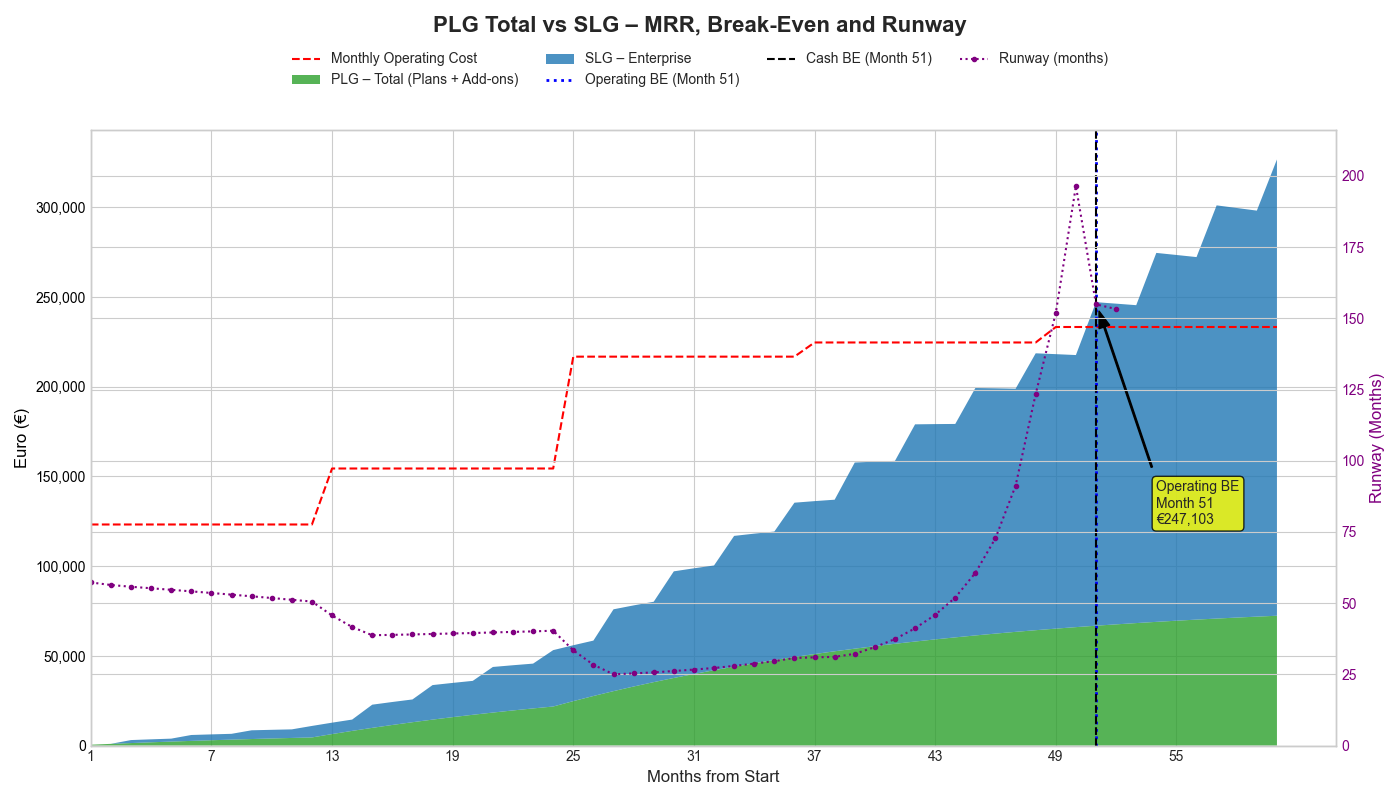
\includegraphics[width=\textwidth]{financial_projection.png}
    \caption{盈亏平衡分析:PLG与SLG MRR、月度成本和营运资金}
    \label{fig:break_even_analysis}
\end{figure} 
\subsection{盈亏平衡分析:图表解读}

\paragraph{图例(速读)}
\begin{itemize}
  \item \textbf{绿色(PLG -- 套餐+附加组件):}自助服务经常性收入。
  \item \textbf{蓝色(SLG -- 企业):}企业经常性收入;由于年度交易在季度间平滑增长,因此按季度“阶梯”增长。
  \item \textbf{红色虚线:}月度运营成本(经审慎调整后),按年以阶梯式增长。
  \item \textbf{紫色点线:}营运资金(月份),计算方法为现金除以3个月移动平均消耗。
  \item \textbf{竖线:}运营盈亏平衡点(蓝色,第51个月)和现金盈亏平衡点(黑色,第51个月)。
\end{itemize}

图表显示了前三年的耐心构建。绿色PLG区域随着月注册量(扣除客户流失后)的复合增长和附加组件带来的增量MRR而稳步上升。蓝色SLG区域随着签订企业合同的签订而以季度以明显的阶梯式增长。成本呈阶梯状变化:每年都会增加增加计划产能(团队、基础设施、一般及管理费用,并包含增长因素),因此红线跳跃然后保持平稳,直到下一步。

这些动态与年终数据相符。第一年末,成本为\textbf{€123{,}212}/月,而经常性MRR为\textbf{€10{,}948}/月(亏损\textbf{€112{,}149}/月,现金\textbf{€5{,}740{,}147},运营周期\textbf{50.6}个月)。第二年末:\textbf{€154{,}413}对比\textbf{€53{,}194}(亏损\textbf{€100{,}855}/月),现金\textbf{€4{,}282{,}549},运营周期\textbf{40.3}个月。第三年末:\textbf{€216{,}746}对比\textbf{€135{,}360}(亏损\textbf{€80{,}631}/月),现金\textbf{€2{,}239{,}361},营运资金\textbf{30.8}个月。收入曲线明显缩小了与成本的差距,同时现金得到控制:\textbf{观察到的最低运营周期为25.0个月},\textbf{峰值月度资金消耗}为\textbf{€160{,}442}。

第四年,差距显著缩小。较大的SLG阶梯使蓝色区域更快扩张,并且(PLG+SLG)的总和几乎达到成本线。年终:成本\textbf{€224{,}646}/月,经常性MRR为\textbf{€218{,}614}/月(总收入\textbf{€219{,}615}/月),接近持平的亏损为\textbf{€5{,}031}/月,现金\textbf{€2{,}239{,}361}。紫色营运资金线开始飙升,因为移动平均资金消耗接近于零。

% ----- End of translated content from: part_15.tex -----

% ----- Start of translated content from: part_16.tex -----

盈亏平衡点出现在\textbf{第51个月}。此时\textbf{经常性MRR为€247{,}103},而成本为\textbf{€233{,}271}(运营盈亏平衡点),\textbf{总收入€248{,}159}超过成本(现金盈亏平衡点)。为了达到这个目标,该模型\textbf{总共消耗€4{,}939{,}370},\textbf{最低现金}为\textbf{€2{,}234{,}573},这也代表着\textbf{盈亏平衡时的储备(占融资轮的30.9\%)}。到第5年末,经常性MRR达到\textbf{€326{,}645/月}($\approx$ \textbf{€3.92M ARR}),月利润为\textbf{€94{,}565},现金为\textbf{€2{,}673{,}539},并且运营期实际上变得无限长。

\paragraph{要点}
图表清晰地展现了三点:
\begin{enumerate}
\item 谁推动了什么 PLG构建基础,SLG弥补差距
\item 为什么成本会随着审慎的运力而大幅上涨
\item 营运资金如何维护 资金周转期从未崩溃(最低25.0个月),而且随着收入增长超过成本,资金周转加速,这和指标报告完全一致。
\end{enumerate}

\begin{table}[H]
\centering
\caption{财务预测摘要(年末)}
\label{tab:financial_summary}
\resizebox{\textwidth}{!}{
\begin{tabular}{lrrrrrrr}
\toprule
\textbf{年末} & \textbf{月度成本(€)} & \textbf{经常性MRR(€)} & \textbf{门店收入(€)} & \textbf{总收入(€)} & \textbf{月度损益(€)} & \textbf{现金余额 €)} & \textbf{运营周期(月)} \\
\midrule
第1年 & 123,212 & 10,948 & 116 & 11,064 & -112,149 & 5,740,147 & 50.6 \\
第2年 & 154,413 & 53,194 & 364 & 53,558 & -100,855 & 4,282,549 & 40.3 \\
第3年 & 216,746 & 135,360 & 755 & 136,115 & -80,631 & 2,823,198 & 30.8 \\
第4年 & 224,646 & 218,614 & 1,001 & 219,615 & -5,031 & 2,239,361 & 123.5 \\
第5年 & 233,271 & 326,645 & 1,191 & 327,836 & 94,565 & 2,673,539 & 收益状态 \\
\bottomrule
\end{tabular}
}
\end{table}

\begin{table}[H]
\centering
\caption{关键财务指标}
\label{tab:financial_metrics}
\resizebox{\textwidth}{!}{%
\begin{tabular}{ll}
\toprule
\textbf{指标} & \textbf{数值} \\
\midrule
运营盈亏平衡点 & 第51个月(第5年):经常性MRR €247,103 $\geq$ 成本 €233,271 \\
盈亏平衡点 & 第51个月(第5年):总收入 €248,159 $\geq$ 成本 €233,271 \\
达到现金盈亏平衡点前已消耗资本 & €4,939,370 \\
月度峰值消耗 & €160,422 \\
期间最低现金 & €2,210,630(占融资轮的30.9\%) \\
最低运营期(3个月移动平均) & 25.0个月 \\
\bottomrule
\end{tabular}
}
\end{table}

\newpage
\section{为什么CNY 59{,}829{,}055是合适的金额}

我们申请的融资金额为\textbf{CNY 59{,}829{,}055} ($\approx€7.15\text{M}$)因为在我们\emph{保守}的预测中, 这笔资金确保公司在不强制增长且保持一定安全裕度的情况下,于51个月实现运营和现金收支平衡。模拟结果明确显示:达到现金盈亏平衡点前累计资金消耗=\textbf{€4{,}939{,}370},盈亏平衡时的现金余额=\textbf{€2{,}210{,}630}(即本轮融资的\textbf{30.9\%}),\textbf{期间最短融资周期=25.0个月}(3个月移动平均值),月度峰值资金消耗=\textbf{€160{,}422}。我们申请的融资金额,符合模型显示,在结构性应急缓冲下达到盈亏平衡所需的必要且充分的金额。

该计划旨在确保韧性:成本并非“基本”,而是按类别(基础设施、一般及管理费用、PLG、SLG、研发、管理)\textbf{审慎增长},以兼顾常被低估的经常性项目(企业支持、审计、法律、招聘、监控)。此外,该模型引入了\textbf{自动防护措施}:如果运营周期低于12个月,则下下个月的可自由支配成本将削减\textbf{10\%};低于9个月,则\textbf{付费PLG收购将被抑制}(乘数0.7)。这些是模型中编码的运营规则,而非承诺。实际上,下行风险自行触发的机制的保护。

在收入方面,我们明确区分\textbf{PLG}(方案+附加组件)和\textbf{SLG}(企业版)。这并非表面文章:它让我们逐月查看支出杠杆的回报率,并且不受意识形态的影戏进行再平衡。通过这种组合和当前价格,\textbf{运营盈亏平衡点}出现在\textbf{第51个月},\textbf{经常性MRR为€247{,}103},而\textbf{月度成本为€233{,}271};在同一个月,由于\textbf{总收入(€248{,}159)}超过成本,因此实现了\textbf{现金盈亏平衡点}。到第5年末,经常性MRR达到\textbf{€326{,}645}($\approx$ \textbf{€3.92M ARR})。就资本效率而言,\textbf{隐含的资金消耗倍数}(盈亏平衡点前的消耗÷盈亏平衡点时的ARR)为\textbf{~1.66倍},这与审慎的产品+市场营销策略以及已经可靠上调的成本相符。

那么,为什么是\emph{这个}金额,而不是更少?如果资金较少,则模型将更频繁地触发防护措机制,从而造成运营上的走走停停(削减/冷却期)尤其是在最需要连续性的时候增加机会成本。为什么不更多呢?因为超过这个门槛,瓶颈不再是预算,而是\textbf{渠道吸收能力}和企业交付的自然节奏;今天的额外现金只会加剧稀释,而不会改善相对于该模型式的结果。

\textbf{筹募的资金用途}仍然与模拟中的类别及其提升保持一致:产品/研发(强化、可观察性、安全性)、基础设施和企业支持、SLG(账户、解决方案/概念验证)、PLG(内容/SDK/社区)、合作伙伴支持、一般及管理费用和合规性、管理。我们不会开设新的支出线:我们按月为模型已经衡量的金额提供资金。

最后,\textbf{风险状况}清晰可读。最低融资期不会低于\textbf{25.0个月},防护机制会在需要时限制现金流失,而\textbf{30.9\%}的盈亏平衡缓冲则为应对采购延迟、基础设施/合规支出波动或汇率波动提供了空间。同时,PLG/SLG分离使得资本配置遵循已实现的回报,而非一刀切的计划——即使事后分析亦如此。

\textbf{简而言之:}\textbf{CNY 59{,}829{,}055}完全满足保守的盈亏平衡运营,并拥有足够的缓冲和自动化的成本控制。这是一个比例合理、可论证的,而且最重要的是\textbf{可复制}可复制的报价:投资者可以逐月验证模型指标是否得到控制,以及现金是否遵循预期的轨迹。

\subsection{战略缓冲的原理:驾驭AI编排领域的先机}
盈亏平衡点时30.9\%的资本储备(€2.21M)代表着我们为应对AI对AI编排市场前所未有的快速变化而做出的深思熟虑的战略配置, 与产品市场契合度遵循可预测模式的传统SaaS领域不同,AI基础设施格局每3-6个月都会经历根本性的变化——从新的LLM架构到新兴的编排标准,如MCP。该缓冲使IntellyHub能够在不影响运营期的前提下快速进行战略调整,无论是适应自主代理能力的突破,集成规划时尚不存在的颠覆性的模型,还是根据实际市场反应在PLG和SLG渠道之间转移重心。成功的AI基础设施公司(Weights \& Biases、Hugging Face)的历史先例表明,该领域的赢家需要经历2-3次重大战略调整才能实现可持续增长——每次调整都会消耗15-20\%的可用资本。我们的储备确保我们能够执行至少一次重大的战略调整, 同时保持12个月以上的运营周期,将原本的生存威胁转变为竞争优势。这不是过剩资金; 而是经过精心计算的期权保险。在一个唯一确定的就是彻底变革的市场中,在竞争对手争相寻求紧急资金的情况下, 能否比竞争对手更快地转型成为市场领导地位和被淘汰之间的决定性因素。

\newpage
\section{市场进入战略}
% Come raggiungerai i tuoi clienti?

IntellyHub的市场进入战略基于混合模式,该模式融合了两个增长引擎:
\begin{enumerate}
    \item \textbf{面向SaaS的产品主导型增长(PLG):} 我们利用产品优势、免费套餐和自动化商店,以可扩展的、自下而上的方式吸引、激活和转化用户。
    \item \textbf{面向本地部署和企业的销售主导型增长(SLG):} 我们采用有针对性的顾问式的销售方式,以赢得具有复杂和安全治理需求的大客户。
\end{enumerate}
这两个引擎旨在相辅相成:PLG策略的成功可为销售团队代来潜在客户和并提升品牌知名度。

% ----- End of translated content from: part_16.tex -----

% ----- Start of translated content from: part_17.tex -----

% --- 战略目标 ---
\subsection{战略目标 (三年期)}
\begin{itemize}
    \item \textbf{定位:} 成为现代技术团队协调复杂自动化和AI工作流程的领先平台。
    \item \textbf{应用:} 在插件生态系统和自动化商店周围达到一定数量的活跃用户和建立充满活力的社区。
    \item \textbf{收入:} 构建一个可持续的商业模式,实现可观的年度经常性收入 (ARR),由 SaaS 订阅和企业本地部署合同驱动。
\end{itemize}


% --- 第一年 ---
\subsection{第一年:基础与市场验证}
\textbf{主要重点:} 赢得早期采用者,验证产品与市场的契合度,并争取首批关键参考客户(SaaS 和本地部署)。在此阶段,许多活动是手动的,并且“无法扩展”。

\newpage
\begin{table}[H]
\centering
\resizebox{\textwidth}{!}{
\begin{tabularx}{\textwidth}{L L L} 
\toprule
\textbf{关键渠道} & \textbf{具体行动} & \textbf{成功关键绩效指标} \\

\midrule
\textbf{产品驱动增长 (PLG)} & 
\textbf{利基市场发布:} 在 Product Hunt、Hacker News 和相关的技术子版块 subreddits(例如 r/devops、r/kubernetes)等平台上展示 IntellyHub。\newline\newline
\textbf{自动化商店:} 在门店中提供 20-30 个高质量的官方模板,用于解决实际的、棘手的问题。
&
\textbf{激活率:} >25\%(用户在 7 天内运行其第一个自动化程序)。\newline\newline
\textbf{1 个月留存率:} >15\%(用户在 4 周后返回)。
\\
\addlinespace

\textbf{技术内容营销} & 
\textbf{博客和教程:} 每月发布 2-4 篇深入的技术文章,展示如何使用 IntellyHub 解决特定问题。\newline\newline
\textbf{视频内容:} 创建简洁的视频教程。
&
\textbf{合格流量:} 来自自然流量和推荐渠道的网站访问量。\newline\newline
\textbf{访客注册率:} >2\%。
\\
\addlinespace

\textbf{社区建设} &
\textbf{Discord/Slack 频道:} 为早期用户建立一个中心枢纽。\newline\newline
\textbf{创始人主导的支持:}  亲自解答每一个问题和反馈请求,以建立良好的关系。
&
\textbf{社区参与度:} 每周活跃会员,点对点支持互动。\newline\newline
\textbf{定性反馈:} 每月至少进行 5 次深入的用户访谈。
\\
\addlinespace

\textbf{创始人主导的销售(内部部署)} &
\textbf{利用网络:} 创始人亲自管理与目标公司在自身人脉中前 3-5 个销售流程。\newline\newline
\textbf{概念验证 (POC):}  关注一些高价值 POC 的成功。
&
\textbf{已启动的概念验证POC:} 全年 3-5 个。\newline\newline
\textbf{已签署的本地合同:} 1-2 个关键参考客户。
\\
\bottomrule
\end{tabularx}
}
\end{table}


% --- 第二年 ---
\newpage
\subsection{第二年:扩张与构建可重复的增长引擎}
\textbf{主要重点:} 将初始价值转化为可扩展、可重复的流程。优化第一年成功经验,并构建商业团队的基础。

\begin{table}[H]
\small
\centering
\resizebox{\textwidth}{!}{
\begin{tabularx}{\textwidth}{L L L}
\toprule
\textbf{关键渠道} & \textbf{具体行动} & \textbf{成功关键绩效指标} \\
\midrule
\textbf{PLG 优化} &

\textbf{漏斗分析:} 使用分析工具识别并消除用户从注册到付费转化过程中的摩擦点。
\textbf{引导式入门:} 打造应用内引导体验,引导新用户找到他们的“顿悟”时刻。
&

% ----- End of translated content from: part_17.tex -----

% ----- Start of translated content from: part_18.tex -----

\textbf{免费到付费转化率:} >3\%。
\textbf{月均经常性收入 (MRR)增长率:}  持续环比增长。
\\
\addlinespace
\textbf{生态系统合作伙伴关系} &

\textbf{战略整合:} 积极为2-3个具有相似用户群的互补技术平台开发插件。
\textbf{联合营销:} 与合作伙伴开展联合营销活动(网络研讨会、博客文章)。
&

\textbf{合作伙伴获取的潜在客户。}
\textbf{合作伙伴插件下载。}
\\
\addlinespace
\textbf{初始销售团队} &

\textbf{首批招聘:}  招聘另一名客户经理来处理潜在客户,并开始有针对性的出战销售。
\textbf{销售策略手册:}  根据创始人领导的销售阶段的经验,规范销售流程。
&

\textbf{每月合格演示次数量。}
\textbf{平均销售周期(本地部署)。}
\\
\bottomrule
\end{tabularx}
}
\end{table}

\newpage
% --- YEAR 3 ---
\subsection{第三年:规模化与细分市场领导力}
\textbf{主要目标:} 加速增长,在技术团队领域占据主导地位,并确立IntellyHub在人工智能为编排市场上的思想领军地位。

\begin{table}[H]
\centering
\resizebox{\textwidth}{!}{
\begin{tabularx}{\textwidth}{L L L}
\toprule
\textbf{关键渠道} & \textbf{具体行动} & \textbf{成功关键绩效指标 (KPI)} \\
\midrule
\textbf{销售规模化} &

\textbf{团队扩张:}  扩大销售团队,覆盖不同的地理区域或行业垂直领域。
\textbf{间接渠道:}  开始探索与系统集成商和经销商的合作。
&

\textbf{年度经常性收入 (ARR)增长。}
\textbf{客户获取成本 (CAC) 和 LTV/CAC 比率。}
\\
\addlinespace
\textbf{品牌营销} &

\textbf{思想领导力:}  基于平台汇总的数据发布和行业报告。
\textbf{赞助:}  赞助DevOps和AI领域的重点会议和播客。
&

\textbf{行业媒体流量效应。}
\textbf{直接流量和品牌流量增长。}
\\
\addlinespace
\textbf{网络效应} &

\textbf{开放商店:}  开放自动化商店和插件市场,向外部合作者认证合作伙伴。
\textbf{开发者计划:}  启动正式的开发者关系 (DevRel) 计划。
&

\textbf{社区创建的插件/模板数量。}
\textbf{净收入留存率 (NRR):}>110\%。
\\
\bottomrule
\end{tabularx}
}
\end{table}

\clearpage
\section{运营计划}
% Come funzionerà l'azienda giorno per giorno.
\subsection{简介}
本文档概述了IntellyHub的开发和市场推广战略的运营计划。该计划与产品开发路线图的各个阶段相一致,并描述了公司各个职能领域的关键活动。

% ----- End of translated content from: part_18.tex -----

% ----- Start of translated content from: part_19.tex -----

% --- 第一阶段 ---
\subsection{第一阶段:基础建设与验证 (第一季度-第二季度)}
\textbf{战略目标:} 将原型转化为稳定安全的最小可行产品 (MVP),获取首批早期用户,并\textbf{通过有针对性的合作伙伴计划验证核心产品和定价模型假设。}

\subsubsection{产品开发与工程}
\begin{itemize}[leftmargin=*]
    \item \textbf{第一季度:}
    \begin{itemize}
        \item \textbf{稳定性:} 完成测试套件(单元测试、集成测试),确保核心引擎的可靠性。
        \item \textbf{插件:} 完成并记录内部系统,以实现标准化插件开发。
        \item \textbf{UI/UX:} 优化混合IDE界面,解决任何同步问题并提升用户体验。
        \item \textbf{本地部署:} 为企业客户开发和测试平台的本地部署版本。
    \end{itemize}
    \item \textbf{第二季度:}
    \begin{itemize}
        \item \textbf{身份验证:} 实施强大的用户管理和身份验证系统。
        \item \textbf{用户引导:} 为新用户开发引导式入门向导。
        \item \textbf{自动化商店 (v1): } 为自动化商店的第一个版 本创建(只读) 的API和UI。
    \end{itemize}
\end{itemize}

\subsubsection{市场营销 (市场营销与销售)}
\begin{itemize}[leftmargin=*]
    \item \textbf{第一季度-第二季度:}
    \begin{itemize}
        \item \textbf{垂直策略:} 在\textit{初始垂直细分市场}(例如,基于Esplorado的用户案例,生物技术/科学研究)中,定义详细的理想客户画像 (ICP)。
        \item \textbf{(新) 设计合作伙伴计划:} 为目标垂直领域中 3-5 家选定的公司启动独家计划
		,提供早期访问和直接支持,以换取持续反馈和潜在的初步合同。
    \end{itemize}
    \item \textbf{第三季度-第四季度:}
    \begin{itemize}
        \item \textbf{细分市场发布:} 在Product Hunt、Hacker News和相关渠道上执行发布,并将沟通重点放在选择的垂直领域。
        \item \textbf{反馈收集:} 收集免费层用户和(优先)设计合作伙伴的结构化反馈。
    \end{itemize}
\end{itemize}

\subsubsection{社区与生态系统管理}
\begin{itemize}[leftmargin=*]
    \item \textbf{第一季度-第二季度:}
    \begin{itemize}
        \item \textbf{定向插件开发:} 开发并记录首批“官方”插件,\textit{优先考虑与目标垂直领域最相关的插件}。
    \end{itemize}
    \item \textbf{第三季度-第四季度:}
    \begin{itemize}
        \item \textbf{社区创建:} 启动官方Discord/Slack服务器。
        \item \textbf{参与:} 创始人及开发团队将积极参与,解答问题并营造友好的环境。
    \end{itemize}
\end{itemize}

\subsubsection{常规运营及公司运营}
\begin{itemize}[leftmargin=*]
    \item \textbf{第一季度-第二季度:}
    \begin{itemize}
        \item \textbf{法律和行政设置:}确定公司构架,开设银行账户。
        \item \textbf{(新) 合作伙伴签约:} 为“设计合作伙伴计划”准备协议。
    \end{itemize}
    \item \textbf{第三季度-第四季度:}
    \begin{itemize}
        \item \textbf{服务条款定义:} 撰写并发布免费套餐的服务条款和隐私政策。
    \end{itemize}
\end{itemize}

\clearpage

% --- 第二阶段 ---
\subsection{第二阶段:扩张与增长 (第三季度-第四季度)}
\textbf{战略目标:} 基于第一阶段验证的数据,扩展用户获取规模,扩展生态系统,并实现盈利所需的企业级功能。

\subsubsection{产品开发与工程}
\begin{itemize}[leftmargin=*]
    \item \textbf{第五季度-第六季度:}
    \begin{itemize}
        \item \textbf{安全性:} 实现凭证的机密管理系统。
        \item \textbf{版本控制:} 为自动化流程添加历史记录和回滚功能。
    \end{itemize}
    \item \textbf{第七季度-第八季度:}
    \begin{itemize}
        \item \textbf{可观察性:} 开发用于流量性能指标的数据平台的第一个版本。
        \item \textbf{改进仪表盘:} 创建用于可视化流程的用户界面。
        \item \textbf{主动人工智能:} 基于流程性能数据实施基本的“自动修复”功能。
    \end{itemize}
\end{itemize}

\subsubsection{市场推广(市场营销与销售)}
\begin{itemize}[leftmargin=*]
    \item \textbf{Q5-Q6:}
    \begin{itemize}
        \item \textbf{垂直内容营销:} 扩大内容制作规模(基于设计合作伙伴的案例研究、文章),重点关注所选垂直领域。
        \item \textbf{招聘:} 开始招聘首位开发者布道师。
    \end{itemize}
    \item \textbf{Q7-Q8:}
    \begin{itemize}
        \item \textbf{付费计划发布:} 完成定价(已通过设计合作伙伴验证)并正式发布专业版和企业版计划。
        \item \textbf{销售策略手册(v1):} 开始为企业客户记录销售流程。
    \end{itemize}
\end{itemize}

\clearpage

% --- PHASE 3 ---
\subsection{第三阶段:领导力与创新(第5-6季度)}
\textbf{战略目标:} 建立市场领导地位,通过社区效应创造网络效应,并\textbf{利用数据建立难以逾越的竞争优势。}

\subsubsection{产品开发与工程}
\begin{itemize}[leftmargin=*]
    \item \textbf{Q9-Q10:}
    \begin{itemize}
        \item \textbf{商店开放:} 开放商店,允许社区提交内容。
        \item \textbf{审核:} 实施内部工具,用于审核和验证外部贡献。
    \end{itemize}
    \item \textbf{Q11-Q12:}
    \begin{itemize}
        \item \textbf{(修订版)数据平台与可观察性:} 开发用于收集和汇总流量绩效指标的系统,战略目标是\textbf{构建“数据护城河”。}
        \item \textbf{分析仪表板:} 创建用于可视化分析的用户界面。
        \item \textbf{主动人工智能:} 改善“自动修复”和主动优化功能,\textbf{基于聚合的平台数据进行训练。}
    \end{itemize}
\end{itemize}

\subsubsection{市场推广(市场营销与销售)}
\begin{itemize}[leftmargin=*]
    \item \textbf{Q9-Q10:}
    \begin{itemize}
        \item \textbf{矿大销售团队规模:} 聘请更多客户经理,负责特定市场或垂直领域。
        \item \textbf{思想领导力:} 开始发布基于平台使用数据的报告和分析。
    \end{itemize}
    \item \textbf{Q11-Q12:}
    \begin{itemize}
        \item \textbf{品牌营销:} 增加对品牌知名度活动的投资(赞助、活动)。
    \end{itemize}
\end{itemize}

\newpage
\section{风险分析}
\subsection{市场风险}
\textit{与市场、竞争和客户采用相关的风险。}

\begin{table}[H]
\centering
\begin{tabularx}{\textwidth}{@{}lL@{}}
\toprule
\textbf{风险} & \textbf{描述} \\
\midrule
\textbf{来自“现状”的竞争} & 我们最大的竞争对手不是替他平台,而是使用自定义Python脚本的开发人员的惯性。他们对脚本的熟悉程度以及 感知到的零初始成本使其成为一个需要克服的重大障碍。 \\
\addlinespace
\textbf{企业采用周期缓慢} & 本地部署和企业销售模式对于高价值合同至关重要,但其特点是销售周期长(6-12个月以上)且概念验证(POC)阶段复杂。首批关键企业交易的延迟可能会显著影响收入预测。 \\
\addlinespace
\textbf{AI技术转型} & 我们目前的人工智能目前被定位为“副驾驶” 果竞争对手若能快速实现技术飞跃,打造出真正自主的、“足够好”的AI代理方面取得快速的技术飞跃,可能会使我们更受控制、更有结构化的方法显得不那么创新。 \\
\bottomrule
\end{tabularx}
\end{table}

\newpage
\subsection{运营风险}
\textit{与技术、人员和执行相关的风险。}

\begin{table}[H]
\centering
\begin{tabularx}{\textwidth}{@{}lL@{}}
\toprule
\textbf{风险} & \textbf{描述} \\

% ----- End of translated content from: part_20.tex -----

% ----- Start of translated content from: part_21.tex -----

\midrule
\textbf{团队执行与关键人员风险} & 该计划依赖于聘用少量高度专业化的高端人才。项目的成功高度依赖于核心团队在产品、基础设施和销售方面的执行能力。关键成员的离职可能会导致严重的延误。 \\
\addlinespace
\textbf{技术复杂性} & 该技术栈(Kubernetes、多步骤AI流水线、混合IDE)功能极其强大,但维护和发展也十分复杂。这个复杂系统中的错误、安全漏洞或性能瓶颈可能难以解决且成本高昂。 \\
\addlinespace
\textbf{混合技术风险(IDE/YAML同步)} & 在复杂的可视化IDE和文本YAML表示之间完美、实时、双向同步在技术上极具挑战性。这可能是潜在的、难以调试的细微错误的来源,可能会影响用户信任。 \\
\addlinespace
\textbf{生态系统质量控制} & 自动化商店和插件市场的价值是一把双刃剑。低质量的、不安全的或维护不善的社区可能会损害用户信任和平台声誉。 \\
\bottomrule
\end{tabularx}
\end{table}

\newpage
\subsection{财务风险}
\textit{与现金流、资金和财务可持续性相关的风险。}

\begin{table}[H]
\centering
\begin{tabularx}{\textwidth}{@{}lL@{}}
\toprule
\textbf{风险} & \textbf{描述} \\
\midrule
\textbf{高初始资金消耗率} & 激进的招聘计划导致在产生可观收入之前,每月运营成本很高。这给实现产品与市场契合度和快速创收带来了巨大压力。 \\
\addlinespace
\textbf{资金依赖} & 商业模式并非为短期盈利而设计。未能达到投资者预期的增长KPI关键绩效指标将构成生存威胁。 \\
\addlinespace
\textbf{定价模式验证} & 提出的价值指标(执行次数、主动自动化)合乎逻辑,但尚未经过验证。错误的定价模式可能导致客户摩擦(如果价格过高)或损失大量收入(如果价格过低)。 \\
\bottomrule
\end{tabularx}
\end{table}

\newpage
\subsection{缓解策略}
\textit{解决和降低已识别风险的具体措施。}

\begin{table}[H]
\centering
\begin{tabularx}{\textwidth}{@{}lL@{}}
\toprule
\textbf{风险类别} & \textbf{缓解策略} \\
\midrule
\textbf{市场风险} & 
\textbf{定位与培训:}市场营销重点并非提花单一脚本, 而是消除长期管理\textit{大量}脚本的长期混乱局面。 使用诸如“Esplorado”等案例研究,提供无可辩驳的价值证明。 \newline\newline
\textbf{混合市场进入策略:}并运行PLG(SaaS)和SLG(本地部署)流程。利用PLG端更快的反馈循环,优化产品和信息传递,以适应较慢的企业销售周期。 \newline\newline
\textbf{战略性AI路线图:}将当前的AI定位为生产环境中务实、安全,可靠的选择。将路线图构建为在现有坚实基础上, 朝着更自主能力发展的演变,。 \\
\addlinespace
\textbf{运营风险} & 
\textbf{文档与交叉培训:}从第一天起就大力投资内部文档。建立知识共享和结对编程的文化,以减少对单个人员的依赖。 \newline\newline
\textbf{投资可观察性和测试:}投入资源构建强大的自动化测试套件,并在早期集成APM(应用程序性能监控)工具,以主动识别和解决问题。该测试套件专门涵盖IDE/YAML同步逻辑。 \newline\newline
\textbf{精选生态系统:}商店初期将仅提供“官方”和“验证合作伙伴”插件。对所有未来的社区提交实施清晰而严格的审查流程,包括自动安全扫描和质量检查。 \\
\addlinespace
\textbf{财务风险} & 
\textbf{基于里程碑的支出:}将支出的大幅增加(尤其是在市场营销和销售人员招聘方面)与实现特定的,预先设定的里程碑(例如,获得前10个付费客户,达到一定的留存率)挂钩。 \newline\newline
\textbf{持续的投资者关系:}与现有和潜在的未来投资者保持透明和定期的沟通渠道,分享KPI关键绩效指标的进展,以建立信心并简化下一轮融资流程。 \newline\newline
\textbf{定价迭代:}采用简单灵活的定价模式。直接与早期客户互动,了解他们获得的价值,并根据他们的反馈和使用数据,准备对定价结构进行迭代。 \\
\bottomrule
\end{tabularx}
\end{table}

\newpage
% \subsection{产品截图}
% 产品的截图、模型图或图表。

\newpage
% 在此处添加文档中引用的任何来源、研究或文章。
\begin{thebibliography}{99}

    \bibitem{AIOrch}
    Market.us, \textit{AI Orchestration Platform Market Report (2024--2034 Forecast)}, February~2025.  
    Available at: \url{https://market.us/report/ai-orchestration-platform-market/}.
    
    \bibitem{GartnerAgentic}
    Reuters (reporting Gartner), \textit{Over 40\% of agentic AI projects will be scrapped by 2027 … by 2028, 33\% of enterprise software will include agentic AI and 15\% of decisions will be made autonomously,} June~25,~2025.
    Available at: \url{https://www.reuters.com/business/over-40-agentic-ai-projects-will-be-scrapped-by-2027-gartner-says-2025-06-25/}.

    \bibitem{MLOpsMM}
    MarketsandMarkets Research, \textit{MLOps Market Size is Anticipated to Cross US\$5.9 Billion by 2027, growing at a CAGR of 41.0\%}, April~21,~2023.
    Available at: \url{https://www.globenewswire.com/news-release/2023/04/21/2652028/0/en/MLOps-Market-Size-is-Anticipated-to-Cross-US-5-9-billion-by-2027-growing-at-a-CAGR-of-41-0-Report-by-MarketsandMarkets.html}.

    \bibitem{ModelOpsGV}
    Grand View Research, \textit{ModelOps Market Report}, 2025 edition.  
    Available at: \url{https://www.grandviewresearch.com/industry-analysis/modelops-market-report}.
    
    \bibitem{langchainGitHub}
    LangChain GitHub Repository.
    Available at: \url{https://github.com/langchain-ai/langchain}

    \bibitem{gartnerAIBarriers}
    Gartner, \textit{2 Barriers to AI Adoption}, November 2, 2021. Available at: \url{https://www.gartner.com/en/articles/2-barriers-to-ai-adoption}

    \bibitem{euAIAct}
    European Commission, \textit{Regulatory framework proposal on artificial intelligence}.
    Available at: \url{https://digital-strategy.ec.europa.eu/en/policies/regulatory-framework-ai}
    
    \bibitem{zapierApps}
    Zapier, \textit{Explore 6,000+ apps}.
    Available at: \url{https://zapier.com/apps}

    \bibitem{g2ZapierReviews}
    G2, \textit{Zapier Reviews}.
    Available at: \url{https://www.g2.com/products/zapier/reviews}

    \bibitem{zapierPricing}
    Zapier, \textit{Zapier Pricing Plans}.
    Available at: \url{https://zapier.com/pricing}

    \bibitem{zapierOpenAI}
    Zapier, \textit{OpenAI Integrations}.
    Available at: \url{https://zapier.com/apps/openai/integrations}

    \bibitem{g2MakeVsZapier}
    G2, \textit{Compare Make vs. Zapier}.
    Available at: \url{https://www.g2.com/compare/make-vs-zapier}

    \bibitem{autogenGitHub}
    Microsoft, \textit{AutoGen GitHub Repository}.
    Available at: \url{https://github.com/microsoft/autogen}

    \bibitem{crewaiGitHub}
    Joao Moura, \textit{CrewAI GitHub Repository}.
    Available at: \url{https://github.com/joaomdmoura/crewAI}

    \bibitem{langchainValuation}
    TechCrunch, \textit{AI infrastructure startup LangChain reportedly raises $100M at $1.1B valuation}, July 9, 2025. Available at: \url{https://siliconangle.com/2025/07/09/ai-infrastructure-startup-langchain-reportedly-raises-100m-1-1b-valuation/#:~:text=Artificial%20intelligence%20infrastructure%2C%20developer%20tools,on%20a%20%241.1%20billion%20valuation.}

    \bibitem{langchainIntegrations}
    LangChain Documentation, \textit{LangChain Integrations}.
    Available at: \url{https://python.langchain.com/docs/integrations/providers/}

    \bibitem{langchainCritique}
    Medium, \textit{Challenges \& Criticisms of LangChain}, March 3, 2025. Available at: \url{https://shashankguda.medium.com/challenges-criticisms-of-langchain-b26afcef94e7}

    \bibitem{mrfRPA}
    Market Research Future, \textit{Robotic Process Automation (RPA) Market Research Report Information By Process (Decision Support, Automated Solution, and Management Solution), By Operations (Rule-based, and Knowledge-based), By Industry (Manufacturing \& Logistics, and IT \& Telecommunication), and By Region (North America, Europe, Asia-Pacific, And Rest of the World) -Industry Size, Share and Forecast Till 2032}.
    Available at: \url{https://www.marketresearchfuture.com/reports/robotic-process-automation-market-2209}

    \bibitem{uipathGartner}
    UiPath, \textit{Gartner Magic Quadrant for RPA}, 2025. Available at:
    \url{https://www.uipath.com/resources/automation-analyst-reports/gartner-magic-quadrant-robotic-process-automation}

    \bibitem{awsSagemaker}
    Amazon AWS SageMaker, \textit{Amazon SageMaker}, Available at: \url{https://aws.amazon.com/sagemaker/}

    \bibitem{forresterRPAvsAI}
    Craig Le Clair, \textit{Will RPA Platforms Remain Relevant? AI Agents May Hold The Answer.}, Forrester, April 25, 2024. Available at: \url{https://www.forrester.com/blogs/will-rpa-platforms-remain-relevant-ai-agents-may-hold-the-answer/}
    
    \bibitem{ChinaAIMarket}
    Grand View Research, \textit{China Artificial Intelligence Market Size \& Outlook}, 2025. Available at: \url{https://www.grandviewresearch.com/horizon/outlook/artificial-intelligence-market/china}

    \bibitem{IntellyHubBP}
    IntellyHub, \textit{Business Plan v2.02}, 2025. Available at: \url{uploaded:businessplan.tex}

    \bibitem{ChinaMLOpsMarket}
    Grand View Research, \textit{China MLOps Market Size \& Outlook, 2024-2030}, 2025. Available at: \url{https://www.grandviewresearch.com/horizon/outlook/mlops-market/china}

    \bibitem{ChinaRPAMarket}
    Grand View Research, \textit{China Robotic Process Automation Market Size \& Outlook}, 2025. Available at: \url{https://www.grandviewresearch.com/horizon/outlook/robotic-process-automation-market/china}

    \bibitem{ChinaProcessOrchMarket}
    Grand View Research, \textit{China Process Orchestration Market Size \& Outlook}, 2022. Available at: \url{https://www.grandviewresearch.com/horizon/outlook/process-orchestration-market/china}

    \bibitem{HyperAutomationShift}
    Fortune Business Insights, \textit{Hyper Automation Market}, 2020. Available at: \url{https://www.fortunebusinessinsights.com/hyper-automation-market-106642}

    \bibitem{HyperAutomationTrends}
    GMI Insights, \textit{Hyper Automation Market Trends}, 2023. Available at: \url{https://www.gminsights.com/industry-analysis/hyper-automation-market}

    \bibitem{APAC_HyperAutomationMarket}
    Market Research Future, \textit{Hyper Automation Market}, 2025. Available at: \url{https://www.marketresearchfuture.com/reports/hyper-automation-market-19259}
    
    \bibitem{NvidiaPreference}
    RAND Corporation, \textit{Leashing Chinese AI Needs Smart Chip Controls}, 2025. Available at: \url{https://www.rand.org/pubs/commentary/2025/08/leashing-chinese-ai-needs-smart-chip-controls.html}

    \bibitem{AlibabaPAI}
    Alibaba Cloud, \textit{What is Machine Learning Platform for AI}, 2025. Available at: \url{https://www.alibabacloud.com/help/en/pai/product-overview/what-is-machine-learning-platform-for-ai/}

    \bibitem{AlibabaCloudInfra}
    Alibaba Cloud, \textit{Machine Learning Products}, 2025. Available at: \url{https://www.alibabacloud.com/en/product/machine-learning?_p_lc=1}

    \bibitem{AlibabaCloudInfra2}
    Alibaba Cloud, \textit{Generative AI Solutions}, 2025. Available at: \url{https://www.alibabacloud.com/en/solutions/generative-ai?_p_lc=1}

    \bibitem{AlibabaQwen}
    Alibaba Cloud, \textit{What is Qwen LLM}, 2025. Available at: \url{https://www.alibabacloud.com/help/en/model-studio/what-is-qwen-llm}

    \bibitem{QwenOpenAIAPI}
    PipeCat.ai, \textit{Qwen LLM Service}, 2025. Available at: \url{https://docs.pipecat.ai/server/services/llm/qwen}

    \bibitem{TencentTI}
    Tencent Cloud, \textit{AI Application Development}, 2025. Available at: \url{https://www.tencentcloud.com/techpedia/119758}

    \bibitem{TencentEcosystem}
    Tencent Cloud, \textit{What is AIOps?}, 2025. Available at: \url{https://www.tencentcloud.com/techpedia/100479}

    \bibitem{TencentEcosystem2}
    Tencent Cloud, \textit{Tencent Cloud Products}, 2025. Available at: \url{https://www.tencentcloud.com/}

    \bibitem{HuaweiModelArts}
    Huawei Cloud, \textit{ModelArts Product Description}, 2025. Available at: \url{https://doc.hcs.huawei.com/modelarts/doc/download/pdf/modelarts-productdesc.pdf}

    \bibitem{HuaweiModelArts2}
    Huawei Cloud, \textit{ModelArts}, 2025. Available at: \url{https://doc.hcs.huawei.com/modelarts/index.html}

    \bibitem{HuaweiModelArts3}
    SourceForge, \textit{Huawei Cloud ModelArts}, 2025. Available at: \url{https://sourceforge.net/software/product/Huawei-Cloud-ModelArts/}

    \bibitem{HuaweiModelArts4}
    Huawei Cloud, \textit{What is ModelArts?}, 2025. Available at: \url{https://support.huawei.com/enterprise/en/doc/EDOC1100328014/6387bf08/what-is-modelarts}

    \bibitem{PaddlePaddleDevs}
    Baidu, \textit{PaddlePaddle}, 2025. Available at: \url{https://www.paddlepaddle.org.cn/en}

    \bibitem{PaddlePaddleToolkits}
    Baidu, \textit{PaddlePaddle Overview}, 2025. Available at: \url{https://www.paddlepaddle.org.cn/en/overview}

    \bibitem{PaddlePaddleEcosystem}
    Viso.ai, \textit{PaddlePaddle: Baidu's Open-Source Deep Learning Platform}, 2025. Available at: \url{https://viso.ai/deep-learning/paddlepaddle/}

    \bibitem{BaiduERNIE}
    Baidu Research, \textit{Announcing the Open Source Release of the ERNIE 4.5 Model Family}, 2025. Available at: \url{https://yiyan.baidu.com/blog/posts/ernie4.5/}

    \bibitem{BaiduERNIE2}
    BotPenguin, \textit{How to Use Baidu Ernie Bot}, 2025. Available at: \url{https://botpenguin.com/blogs/how-to-use-baidu-ernie-bot}

    \bibitem{MakeAlternatives}
    Appy Pie, \textit{10 Best Make (Formerly Integromat) Alternatives in 2025}, 2025. Available at: \url{https://appypieautomate.ai/blog/alternatives/make-alternatives}

    \bibitem{MakeAlternatives2}
    Lindy.ai, \textit{12 Best Make Alternatives for AI Automation in 2025}, 2025. Available at: \url{https://www.lindy.ai/blog/make-alternatives}

    \bibitem{MakeVsZapier}
    Knack, \textit{Make.com vs Zapier (Comparison Guide 2025)}, 2025. Available at: \url{https://www.knack.com/blog/make-com-vs-zapier-comparison-guide-2025/}

    \bibitem{MendixChina}
    AppMaster, \textit{Mendix Enters the Chinese Market with its Low-Code Application Platform}, 2025. Available at: \url{https://appmaster.io/it/news/mendix-entra-nel-mercato-cinese-con-la-sua-piattaforma-applicativa-low-code}

    \bibitem{DingTalkAI}
    DeepSeek AI, \textit{Awesome DeepSeek Integration}, 2025. Available at: \url{https://github.com/deepseek-ai/awesome-deepseek-integration}

    \bibitem{DingTalkAPI}
    MCP Market, \textit{Dingding MCP Server}, 2025. Available at: \url{https://mcpmarket.com/server/dingding}

    \bibitem{LangChainAlternatives}
    IPRoyal, \textit{8 Best LangChain Alternatives for Building LLM Apps}, 2025. Available at: \url{https://iproyal.com/blog/langchain-alternatives/}

    \bibitem{AIAgentFrameworks}
    Langfuse, \textit{AI Agent Frameworks Comparison: LangChain, CrewAI, AutoGen, Semantic Kernel, and LlamaIndex Agents}, 2025. Available at: \url{https://langfuse.com/blog/2025-03-19-ai-agent-comparison}

    \bibitem{ChineseLLMs}
    Index.dev, \textit{Top 5 Chinese Open-Source LLM Models}, 2025. Available at: \url{https://www.index.dev/blog/chinese-open-source-llms}

    \bibitem{DataLocalization}
    Future of Privacy Forum, \textit{Demystifying Data Localization: A Guide for Global Businesses Navigating China's Data Security Regime}, 2022. Available at: \url{https://fpf.org/wp-content/uploads/2022/02/Demystifying-Data-Localization-Report.pdf}

    \bibitem{PIPLSummary}
    DLA Piper, \textit{Data Protection Laws of the World: China}, 2025. Available at: \url{https://www.dlapiperdataprotection.com/index.html?c=CN}

    \bibitem{PIPLImpact}
    PwC, \textit{China's new data privacy law: What it means for your business}, 2021. Available at: \url{https://www.pwc.com/us/en/tech-effect/cybersecurity/china-pipl-rules-impact.html}

    \bibitem{CSL}
    Wikipedia, \textit{Cybersecurity Law of the People's Republic of China}, 2025. Available at: \url{https://en.wikipedia.org/wiki/Cybersecurity_Law_of_the_People%27s_Republic_of_China}

    \bibitem{CrossBorderData}
    California Lawyers Association, \textit{Cross-Border Data Transfer Mechanism in China and its Compliance}, 2023. Available at: \url{https://calawyers.org/business-law/cross-border-data-transfer-mechanism-in-china-and-its-compliance/}

    \bibitem{DataLocalizationImportance}
    EdgeNext, \textit{What is the importance of data localization in China \& how can CDNs help?}, 2024. Available at: \url{https://www.edgenext.com/what-is-the-importance-of-data-localization-in-china-how-can-cdns-help/}

    \bibitem{PIPLConsent}
    China Briefing, \textit{China's PIPL: A Guide for Foreign Businesses}, 2024. Available at: \url{https://www.china-briefing.com/doing-business-guide/china/company-establishment/pipl-personal-information-protection-law}

    \bibitem{GenAIInterimMeasures}
    PwC, \textit{Interim Measures for the Management of Generative Artificial Intelligence Services officially implemented}, 2023. Available at: \url{https://www.pwccn.com/en/tmt/interim-measures-for-generative-ai-services-implemented-aug2023.pdf}

    \bibitem{GenAIRegsFinal}
    Data Protection Report, \textit{China finalises its generative AI regulation}, 2023. Available at: \url{https://www.dataprotectionreport.com/2023/07/china-finalises-its-generative-ai-regulation/}

    \bibitem{GenAIRegsFinal2}
    Hogan Lovells, \textit{China finalizes generative AI regulation}, 2023. Available at: \url{https://www.hoganlovells.com/en/publications/china-finalizes-generative-ai-regulation}

\end{thebibliography}


\end{document}